%Dies ist die Hauptseite des Dokumentes. Es werden u. a. alle Kapitel,
%Einstellung im Header eingebunden.  Veränderungen müssen in folgenden Dateien
%vorgenommen werden:
      %- config.tex
      %- einzelne Kapitel (evtl. erweitern)

%Hier sind alle Einstellungen enthalten, die sich auf das Seiten- und
%Dokumentenlayout beziehen

\documentclass[
  11pt,                   % Schriftgröße
  DIV12,
  german,                 % für Umlaute, Silbentrennung etc.
  oneside,                % einseitiges Dokument
  titlepage,              % es wird eine Titelseite verwendet
  parskip=half,           % Abstand zwischen Absätzen (halbe Zeile)
  headings=normal,        % Größe der Überschriften verkleinern
  captions=tableheading,  % Beschriftung von Tabellen unterhalb ausgeben
  final                   % Status des Dokuments (final/draft)
]{scrreprt}               %


%------Ändern von Schriftschnitten - (Muss ganz am Anfang stehen !) ------------
\usepackage{fix-cm}


%------Umlaute -----------------------------------------------------------------
%   Umlaute/Sonderzeichen wie äüöß können direkt im Quelltext verwenden werden.
%    Erlaubt automatische Trennung von Worten mit Umlauten.
\usepackage[T1]{fontenc}
\usepackage[utf8]{inputenc}

%------Anpassung der Landessprache----------------------------------------------
\usepackage[ngerman]{babel}

%------Einfache Definition der Zeilenabstände und Seitenränder------------------
\usepackage{geometry}
\usepackage{setspace}

%------Schriftgrößenanpassung von einzelnen Textpassagen------------------------
\usepackage{relsize}

%------Trennlinien in Kopf- und Fusszeile
\usepackage[headsepline, footsepline, ilines]{scrpage2}

%------Grafiken und Farben -----------------------------------------------------
\usepackage{xcolor}
\usepackage{graphicx}

%------Packet zum Sperren, Unterstreichen und Hervorheben von Texten------------
\usepackage{soul}

%------ergänzende Schriftart----------------------------------------------------
\usepackage{helvet}

%------Lange Tabellen-----------------------------------------------------------
\usepackage{longtable}
\usepackage{array}
\usepackage{ragged2e}
\usepackage{lscape}

%------PDF-Optionen-------------------------------------------------------------
\usepackage[
  bookmarks,
  bookmarksopen=true,
  colorlinks=true,
  linkcolor=black,        % einfache interne Verknüpfungen
  anchorcolor=black,      % Ankertext
  citecolor=black,        % Verweise auf Literaturverzeichniseinträge im Text
  filecolor=black,        % Verknüpfungen, die lokale Dateien öffnen
  menucolor=black,        % Acrobat-Menüpunkte
  urlcolor=black,         % Farbe für URL-Links
  backref,                % Zurücktext nach jedem Bibliografie-Eintrag als
                          % Liste von Überschriftsnummern
  pagebackref,            % Zurücktext nach jedem Bibliografie-Eintrag als
                          % Liste von Seitenzahlen
  plainpages=false,       % zur korrekten Erstellung der Bookmarks
  pdfpagelabels,          % zur korrekten Erstellung der Bookmarks
  hypertexnames=false,    % zur korrekten Erstellung der Bookmarks
  linktocpage             % Seitenzahlen anstatt Text im Inhaltsverzeichnis verlinken
  ]{hyperref}






      % enthält eingebundene Packete

%------Seitenränder-------------------------------------------------------------
\geometry{verbose,                     % zeigt die eingestellten Parameter beim
                                       % Latexlauf an
      paper=a4paper,                   % Papierformat
      top=25mm,                        % Rand oben
      left=25mm,                       % Rand links
      right=25mm,                      % Rand rechts
      bottom=45mm,                     % Rand unten
      pdftex                           % schreibt das Papierformat in die
                                       % Ausgabe damit Ausgabeprogramm
                                       % Papiergröße erkennt
  }

%Seitenlayout
\onehalfspace        % 1,5-facher Abstand

%------Kopf- und Fußzeilen -----------------------------------------------------
\pagestyle{scrheadings}

%------Kopf- und Fußzeile auch auf Kapitelanfangsseiten ------------------------
\renewcommand*{\chapterpagestyle}{scrheadings}

%------Schriftform der Kopfzeile -----------------------------------------------
\renewcommand{\headfont}{\normalfont}

%----Spezielle Befehle
\newcommand{\lfk}[1]{$\langle LF#1\rangle$}

%----Farben
\definecolor{tubsRed}{cmyk}{0.1,1.0,0.8,0.0}
\definecolor{tuRed}{cmyk}{0.1,1.0,0.8,0.0}

%------Kopfzeile----------------------------------------------------------------
\setheadsepline{1pt}[\color{tuRed}]
\setlength{\headheight}{21mm}        % Höhe der Kopfzeile
\ihead{\large{\textsc{\praktikumTitel}}\\    % Text in der linken Box
       \small{\projektTitel}}
\chead{}                            % Text in der mittleren Box

%----Fusszeile
\setfootsepline{1pt}[\color{tuRed}]
\cfoot{}                            % Text in mittlerer Box
\ofoot{\pagemark}                    % Seitenzahl in rechter Box



%------Labels mit eigenem Text für \ref ----------------------------------------
\makeatletter
\def\namedlabel#1#2{\begingroup
#2%
\def\@currentlabel{#2}%
\phantomsection\label{#1}\endgroup
}
\makeatother


%------Neue Environments -------------------------------------------------------

\newcommand{\refsetcounter}[2]{\setcounter{#1}{#2}\addtocounter{#1}{-1}\refstepcounter{#1}}

%Funktion im Pflichtenheft
\newcounter{functioncount} 
\newenvironment{function}[2]{\refsetcounter{functioncount}{#1}\large\textbf{\sffamily{#2 }}\namedlabel{F#1}{$\langle F#1\rangle$}\normalsize\begin{description}\setlength{\itemsep}{-5pt}}{\end{description}}

%Daten im Pflichtenheft
\newcounter{datacount} 
\newenvironment{data}[2]{\refsetcounter{datacount}{#1}\textbf{#2} \namedlabel{D#1}{$\langle D#1\rangle$}\\}{}

%Kriterien im Pflichtenheft
\newcounter{mustcount} 
\newcommand{\must}[2]{\refsetcounter{mustcount}{#1}\namedlabel{RM#1}{$\langle RM#1\rangle$} #2\\}

\newcommand{\should}[2]{\refsetcounter{datacount}{#1}\namedlabel{RS#1}{$\langle RS#1\rangle$} #2\\}

\newcommand{\could}[2]{\refsetcounter{datacount}{#1}\namedlabel{RC#1}{$\langle RC#1\rangle$} #2\\}

\newcommand{\wont}[2]{\refsetcounter{datacount}{#1}\namedlabel{RW#1}{$\langle RW#1\rangle$} #2\\}

%Qualitätsanforderungen im Pflichtenheft
\newcommand{\qualityReq}[2]{\refsetcounter{datacount}{#1}\namedlabel{Q#1}{$\langle Q#1\rangle$} #2\\}

% Benutzeroberflächen im Pflichtenheft
\newcounter{uicount}
\newenvironment{ui}[2]{\refsetcounter{uicount}{#1}\textbf{#2} \namedlabel{UI#1}{$\langle UI#1\rangle$}\\}{}

% Klassen
\newcounter{classcount}
\newenvironment{class}[2]{\refsetcounter{classcount}{#1}\textbf{#2}\namedlabel{CL#1}{$\langle CL#1\rangle$}\begin{description}\setlength{\itemsep}{-5pt}}{\end{description}}

% Entitäten
\newcounter{entitycount}
\newenvironment{entity}[2]{\refsetcounter{entitycount}{#1}\textbf{#2} \namedlabel{E#1}{$\langle E#1\rangle$}\\}{}

% Component
\newcounter{componentcount}
\newenvironment{component}[2]{\refsetcounter{componentcount}{#1}\textbf{Komponente \namedlabel{C#1}{$\langle C#1\rangle$}: #2}\\}{}

% Interface
\newcounter{interfacecount}
\newenvironment{interface}[2]{\refsetcounter{interfacecount}{#1}\textbf{Schnittstelle \namedlabel{I#1}{$\langle I#1\rangle$}: #2}\\}{}

% Testfall
\newcounter{testcasecount}
\newenvironment{testcase}[2]{\clearpage\refsetcounter{testcasecount}{#1}\subsection{Testfall $\langle T#1\rangle$ - #2}\label{T#1}\begin{description}\setlength{\itemsep}{-5pt}}{\end{description}}
          % Diese Datei enthält alle
                                          % Layouteinstellungen
\newcommand{\dokumentTitel}{Fachentwurf}
% Definition von globalen Parametern, die derzeit auf der Titelseite und in der
% Kopfzeile verwendet werden. Der in <> gesetzte Text ist zu verändern.

\newcommand{\praktikumTitel}{Das Gro\ss{}e SQL-Spiel}
\newcommand{\projektTitel}{The SQL-Alchemist}
\newcommand{\institut}{
	Institut f\"ur Informationssysteme\\
	Prof. Dr. Wolf-Tilo Balke\\
	M\"uhlenpfordtstra\ss{}e 23, 2.OG\\
	D-38106 Braunschweig\\
}
\newcommand{\institutsLogo}{common/ISF_Logo.pdf}
\newcommand{\betreuer}{Jan-Christoph Kalo}


%------Beginn des Gesamtdokumentes----------------------------------------------
\begin{document}

%------Eingebundene Seiten, Verzeichnisse bzw. Kapitel--------------------------
% Dies ist die Titelseite.
% Die Ausgabe darf 1 Seite nicht überschreiten, also ggf. Abstände anpassen
% Die Angabe in [...] gibt den Abstand nach der entsprechenden Zeile an.


%----Stil dieser Seite----------------------------------------------------------
\thispagestyle{plain}      % Kopfzeile bleibt leer

%----Beginn der Titelseite------------------------------------------------------
\begin{titlepage}

%----eingebundenes Logo der TU--------------------------------------------------
%\setlength{\unitlength}{1mm}
%  \begin{picture}(00,00)(+25,-04)
%  	\color{tuRed}
%    \put(055,006){\line(1,0){150}}
%    \put(005,000){
\includegraphics[width=6.3cm]{common/TUBraunschweig_4C.pdf}}
%    \put(150,010){\includegraphics[width=8cm,height=2.4cm,keepaspectratio]{\institutsLogo}}
%  \end{picture}\\[5ex]
%\hspace*{-2cm}


\vspace*{-3.8cm}
\hspace*{-2cm}\begin{minipage}{1.25\textwidth}

\includegraphics[width=6.3cm]{common/TUBraunschweig_4C.pdf}\setlength{\unitlength}{1mm}\begin{picture}(00,00)(0,0)\color{tuRed}\put(000,004){\line(1,0){150}}\end{picture}%\hfill
\parbox[b]{0.68\textwidth}{\hfill\includegraphics[width=8cm,height=2.4cm,keepaspectratio]{\institutsLogo}\\~}
\end{minipage}


~\\[4ex]

%----zentrierte Ausrichtung über die gesamte Seite----------------------------
\begin{center}

%----Titel des Praktikum (\praktikumTitel in newComments zu verändern)--------
{\relsize{4}{\textbf{\textsc{\praktikumTitel}}}}\\[4ex]

%----Titel des Teilprojektes (\projektTitel in newComments verändern)---------
{\relsize{3}{\textbf{\textsc{\projektTitel}}}}\\[4ex]

Software-Entwicklungspraktikum (SEP)\\
Sommersemester 2015\\[4ex]

{\relsize{3}{\textbf{\dokumentTitel}}}\\[2ex]

%----Daten des Auftraggebers
Auftraggeber:\\
Technische Universität Braunschweig\\
\institut[2ex]
Betreuer: \betreuer\\[2ex]

Auftragnehmer:\

% ----Tabelle der Praktikumsteilnehmer------------------------------------------
\begin{tabular}{l<{\hspace{20mm}} l<{\hspace{21mm}}}\\

  Name                   &   E-Mail-Adresse\\      % Zeilenüberschift

  \hline                    % Linie unterhalb der Zeilenüberschrift

  %----Nachfolgend alle Namen und E-Mail-Adressen der Teilnehmer einfügen
 
 Gabriel Ahlers &  g.ahlers@tu-braunschweig.de\\
 Majid Dashtiepielehroud &  m.dashtiepielehroud@tu-braunschweig.de\\
 Ronja Friebe &  r.friebe@tu-braunschweig.de\\  
 Stefan Hanisch &  stefan.hanisch@tu-braunschweig.de\\  
 Fabio Luigi Mazzone & f.mazzone@tu-braunschweig.de\\  
 Nicole Naczk &  n.naczk@tu-braunschweig.de\\  
 Denis Nagel &  denis.nagel@tu-braunschweig.de\\  
 Luca Porcello &  l.porcello@tu-braunschweig.de\\  
 Christian Reineke &  c.reineke@tu-braunschweig.de\\  
 Christian Sander &  christian.sander@tu-braunschweig.de\\  
 Carl Schiller &  c.schiller@tu-braunschweig.de\\  
 Levent Muzaffer \"Uner &  l.uener@tu-braunschweig.de\\  
 S\"oren van der Wall &  s.van-der-wall@tu-braunschweig.de\\  
 Daniel Wolfram &  d.wolfram@tu-braunschweig.de\\  


\end{tabular}

%Zur Vereinheitlichung sollten hier die TU Braunschweig Emailadressen benutzt werden. % enthält Tabelle der Praktikumsteilnehmer

\vfill
Braunschweig, \today

\end{center}
\end{titlepage}
                      % Titelseite


\tableofcontents                          % Inhaltsverzeichnis wird automatisch
                                          % generiert
\listoffigures                            % ebenso das Abbildungsverzeichnis

%----Kapitel des Fachlichen Entwurfs, die mit Inhalt zu füllen sind--------------------
%!TEX root = ../Fachentwurf.tex

\chapter{Einleitung}
Ziel dieses Dokuments ist es, einen tiefer gehenden Überblick über den internen Ablauf der zu entwickelnden Software zu bieten. Es werden zuerst die wichtigsten Funktionen einzeln beschrieben, wobei Sequenzdiagramme zu Hilfe genommen werden. Danach wird die Datenverwaltung näher beleuchtet. \\

\begin{figure}[h]
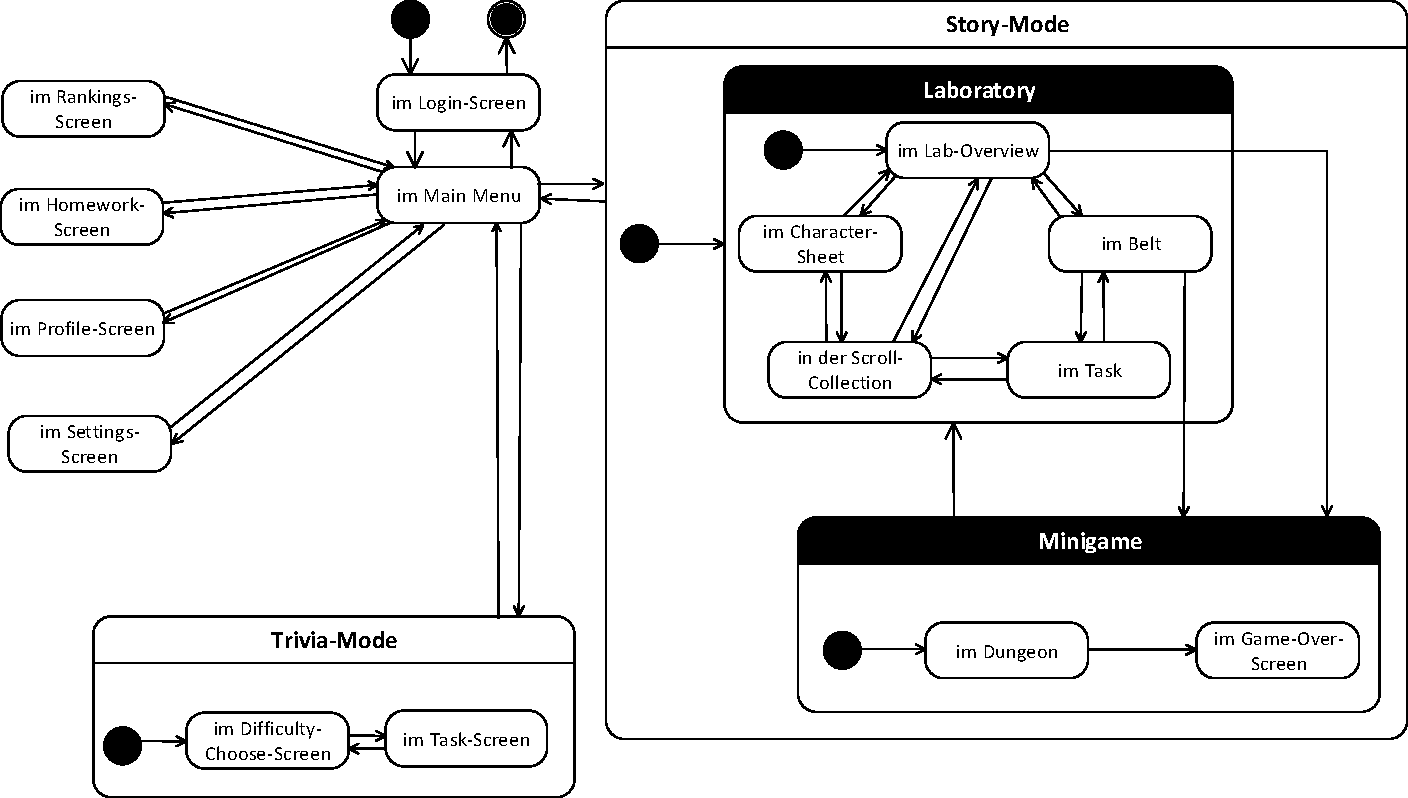
\includegraphics[width=1.0\textwidth]{figures/statechart_game.pdf}
\caption{Zustandsdiagramm zum oberflächlichen Spielablauf}
\label{sequence}
\end{figure}


Um eine Verständnisgrundlage zu schaffen ist in Abbildung 1.1 der allgemeine Men\"uf\"uhrung in einem Aktivit\"atsdiadramm dargestellt. 


Nach dem Einloggen gelangt man in das Main Menu. Von dort aus gelangt man in die drei Spielmodi (Story, Trivia, Homework), die Einstellungen, das Profil und in die Ranglisten.

Der Story Mode hat wiederum eine eigene Übersicht, Laboratory genannt. Von hier aus kann der User sich seine aktuellen Playerstatistiken im Charakter Sheet ansehen, kann sich in der Scrollcollection um die Herstellung von Potions und Enchantments k\"ummern, diese danach in seinen Belt einf\"ugen um sich im Anschluss dem Minispiel zu widmen. Im Minispiel werden dem User verschiedene Hindernisse vorgesetzt, die es zu überwinden gilt. Scheitert der User, so gelangt er in den Game Over Screen, in dem ihm angezeigt wird wie viele Lofi-Coins (die Spiel-Währung) und welche Scrolls er in dieser Runde eingesammelt hat. Nach Bestätigung befindet sich der User zurück im Laboratory.

Der Trivia-Mode stellt einen SQL-Trainer dar. Entscheidet der User sich dafür diesem zu verwenden, gelangt er in einen Screen in dem er sich für einen Schwierigkeitsgrad entscheiden muss. Hat der User dies getan, erhält er eine, dem ausgewählten Schwierigkeitsgrad entsprechende, Aufgabe und kann diese lösen.

Der Homework-Mode funktioniert genauso wie der Trivia-Mode, lediglich die Auswahl des Schwierigkeitsgrads entf\"allt in diesem Fall.

In den Rankings werden die Spieler nach verschiedenen Kriterien in Ranglisten sortiert. Darüber ist es auch möglich durch die Eingabe des Usernamens nach anderen Spielern zu suchen und sich deren Profile anzeigen zu lassen.
Das eigene Profil ist über das Main Menu zu erreichen und einsehbar. Selbiges gilt für die Spieleinstellungen.  



\section{Projektdetails}

Die Anzahl an Lofi-Coins, sowie die Anzahl an Scroll die der User pro Tag einsammeln kann, werden beschr\"ankt.
Dies soll verhindern, dass der User nicht den Fokus, des \"Ubens von SQL-Statements, verliert. Auf der anderen Seite jedoch, soll so der Spieler zum Wiederkommen
animiert werden.

Desweiteren wurde im Pflichtenheft erwähnt, dass Spieler sich durch Aufgabenerstellung ins Spiel mit einbringen können. Um dabei jedoch eine gewisse Qualität zu gewährleisten zu k\"onnen, wird es nur beförderten Nutzern möglich sein, eigene Aufgaben zu erstellen. Wie ein User befördert wird, wird über die Spielzeit oder über Leistungen im Spiel geregelt.  

%Besonders interessante oder komplizierte Sachverhalte sollen hier noch weiter vertieft werden.
 %Auch hier sollen Aktivitätsdiagrame und Statecharts verwendet werden.

%Beispiele:
%\begin{itemize}
%\item Bei einem Spiel könnten komplizierte Regeln dargestellt werden.
%\item In einen Web-System könnte bestimmte Workflows als Aktivitätsdiagramm dargestellt werden.
%\end{itemize}

%Es kann pro Sachverhalt ein Abschnitt hinzugefügt werden.


%!TEX root = ../Fachentwurf.tex

\chapter{Analyse der Produktfunktionen}\label{chap:analyse}
Im Folgenden werden die im Pflichtenheft benannten Funktionen näher beschrieben und erkl\"art. Dabei wird davon ausgegangen, dass der User sich in dem Interface befindet, in dem er die erklärte Funktion initiieren kann.

Desweiteren ist zu erkennen, dass, jedes mal wenn das Back-End nach der Registration oder dem Login aktiv wird, es zuerst einen \glqq checkSession()\grqq -Methodenaufruf startet. Dies ist die Überprüfung des Back-Ends, ob es selbst den User kennt, ob er die gebrauchten Rechte für die Aktion hat und ob die Aktion auch auf die zum User gehörigen Daten ausgeführt wird.

\newpage
\section{Analyse von Funktionalität <F10>: <Nutzer registrieren>}
\begin{figure}[htb]
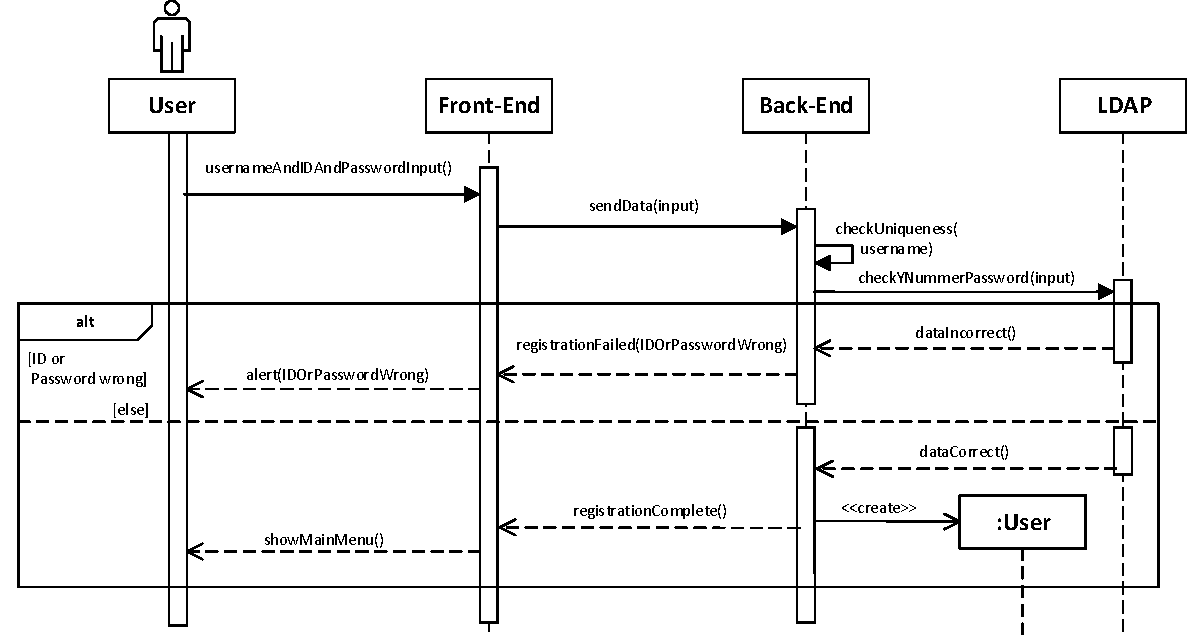
\includegraphics[width=1.3\textwidth]{figures/sequenz_F10.pdf}
\caption{Sequenzdiagramm zur Registrierung}
\label{sequence}
\end{figure}


\newpage
In Diagramm 2.1 wird der Vorgang der Registrierung beschrieben.

Dafür muss der User zuerst einen Username, eine E-Mail-Adresse oder seine y-Nummer (insgesamt ID genannt) und ein Passwort (im Falle einer y-Nummer das zur y-Nummer gehörende Passwort) angeben. Diese Eingaben werden dann an das Back-End übertragen. Hier wird zuerst geprüft ob der Username schon vergeben ist. Sollte das der Fall sein, wird dies dem User mitgeteilt und er muss einen neuen Username angeben.
Wenn der Username noch nicht vergeben war, wird, sollte die ID eine E-Mail-Adresse sein, geprüft, ob diese schon vorhanden ist. Wenn die ID eine y-Nummer ist wird diese inklusive des eingegebenen Passworts an das \glqq LADP\grqq geschickt und dort überprüft. Sollte der jeweils zutreffende Schritt fehlschlagen, muss der User seine Eingaben ändern beziehungsweise korrigieren und der Prozess beginnt von vorn.

Sollte der Ablauf erfolgreich verlaufen sein, erstellt das Back-End ein neues User-Objekt, speichert dies in seiner Datenbank und gibt die Rückmeldung, dass die Registrierung erfolgreich verlaufen ist und der User wird in das Hauptmenü weitergeleitet.
%==================================================================

\newpage
\section{Analyse von Funktionalität <F20>: <Nutzer anmelden>}
\begin{figure}[h]
\centering
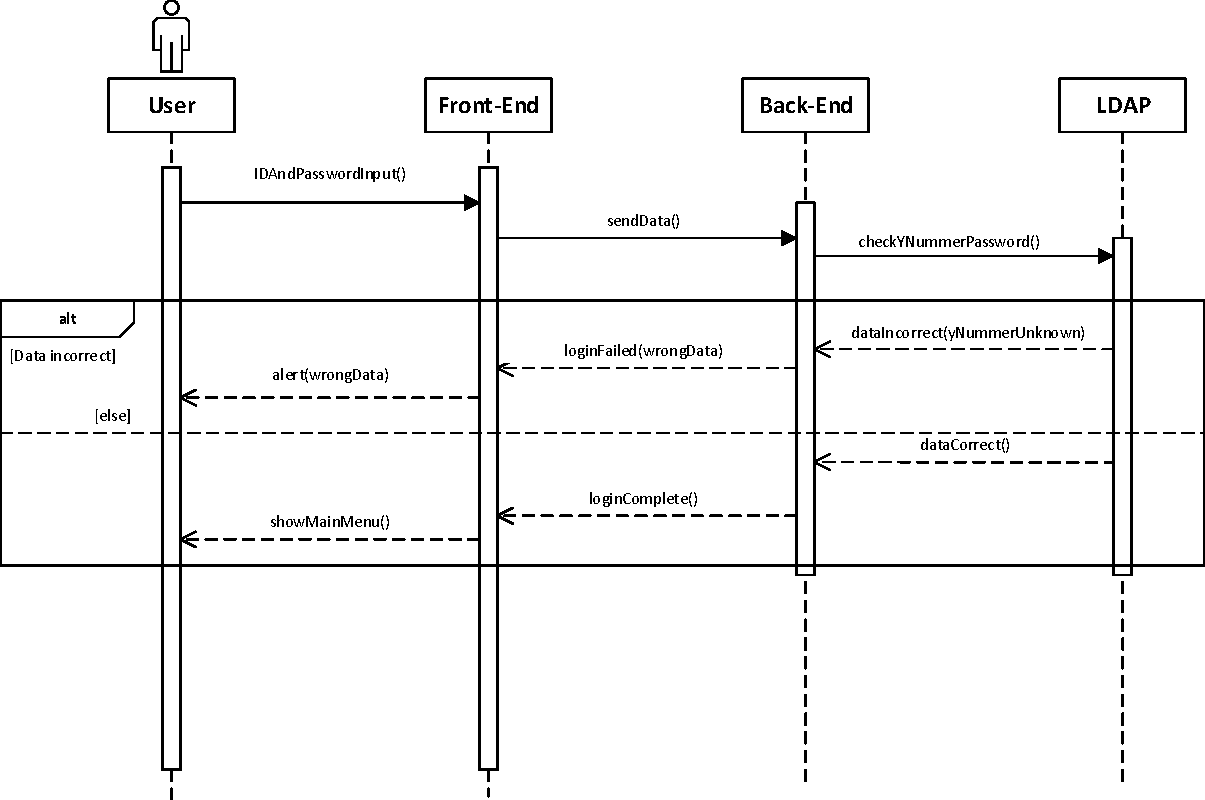
\includegraphics[width=1.3\textwidth]{figures/sequenz_F20.pdf}
\caption{Sequenzdiagramm zum Login}
\label{sequence}
\end{figure}
Das Diagramm 2.2 beschreibt den Login-Vorgang. 

Hierbei muss der User die von ihm registrierte ID (siehe <F10>) und sein Passwort angeben. Diese werden, je nach Typ der ID, dann entweder mit der eigenen Datenbank verglichen, oder, sollte die ID eine y-Nummer sein, an das \glqq LDAP\grqq geschickt und dort überprüft.
Sollten die eingegeben Daten nicht korrekt sein, wir dies dem User mitgeteilt und er bekommt die Möglichkeit seine Eingaben zu korrigieren. Sind die Daten korrekt wird der User in das Hauptmenü weitergeleitet.
%==================================================================

\newpage
\section{Analyse von Funktionalität <F30>: <Nutzer abmelden>}
\begin{figure}[h]
\centering
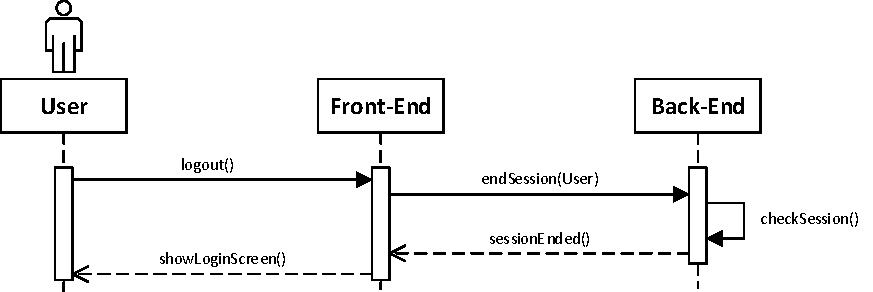
\includegraphics[width=1.4\textwidth]{figures/sequenz_F30.pdf}
\caption{Sequenzdiagramm zum Login}
\label{sequence}
\end{figure}
Das Diagramm 2.3 beschreibt den Ablauf des Ausloggens.

Entscheidet sich der User sich auszuloggen, wir diese Information an das Back-End gesendet. Dieses beendet die Session des Users. Ist das geschehen wird eine Benachrichtigung an das Front-End gesendet und der User wird zurück zum Login-Screen geleitet.
%==================================================================

\newpage
\section{Analyse von Funktionalität <F40>: <Profil einsehen>}
\begin{figure}[h]
\centering
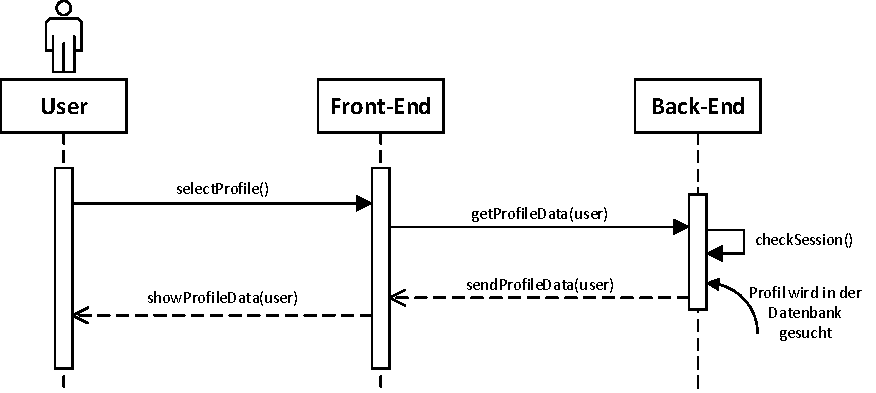
\includegraphics[width=1.3\textwidth]{figures/sequenz_F40.pdf}
\caption{Sequenzdiagramm zur Darstellung der Profilübersicht}
\label{sequence}
\end{figure}
Das Diagramm 2.4 zeigt was passiert, wenn man sich das eigene Userprofil anzeigen lassen möchte.

Um das Profil des Users anzuzeigen werden zuerst die Userdaten vom Back-End angefordert. Das Back-End lädt dann die Profildaten aus den Userdaten und schickt diese zurück an das Front-End. Dort werden sie für den User einsehbar im Profil-Interface angezeigt.

%==================================================================

\newpage
\section{Analyse von Funktionalität <F60>: <Passwort ändern>}
\begin{figure}[h]
\centering
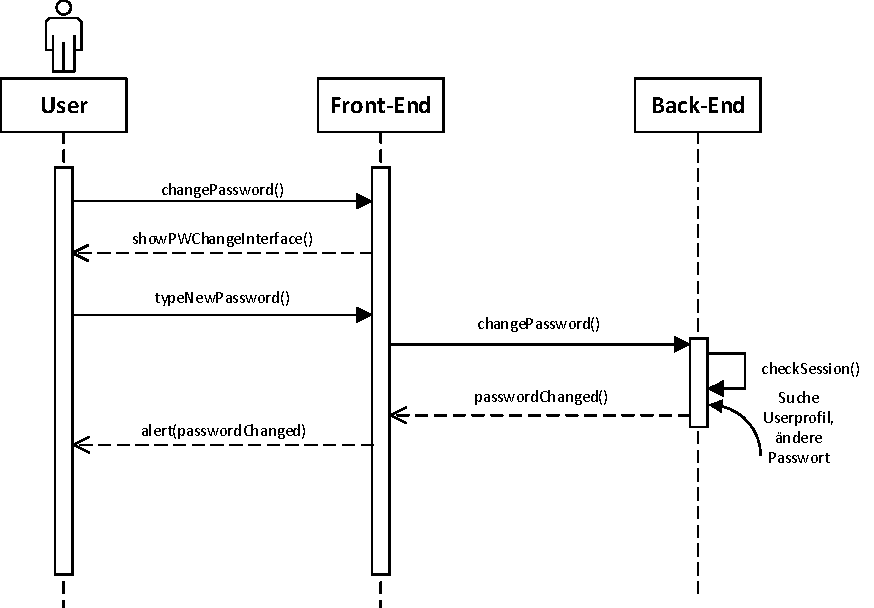
\includegraphics[width=1.3\textwidth]{figures/sequenz_F60.pdf}
\caption{Sequenzdiagramm zum Ändern des Passworts}
\label{sequence}
\end{figure}
Das Diagramm 2.5 beschreibt das Ändern des Passwortes.

Das Ändern des Passwortes steht nur nicht-studentischen Nutzern zur Verfügung.
Entscheidet sich der Nutzer, sein Passwort zu ändern, kann er dies mit einem Klick auf den Change Password Button tun. Zuerst muss er sein altes Passwort eingeben und im Anschluss kann er ein neues Password erstellen. Dies muss danach noch einmal bestätigen werden und wenn alles erfolgreich war, wird das geänderte Passwort an das Back-End geschickt und dort in den Nutzerdaten vermerkt. Sollte während des Vorgangs etwas schief gehen, bleibt das alte Passwort bestehen und der User wird darüber in Kenntnis gesetzt.
%==================================================================

\newpage
\section{Analyse von Funktionalität <F70>: <Avatar ändern>} 
\begin{figure}[h]
\centering
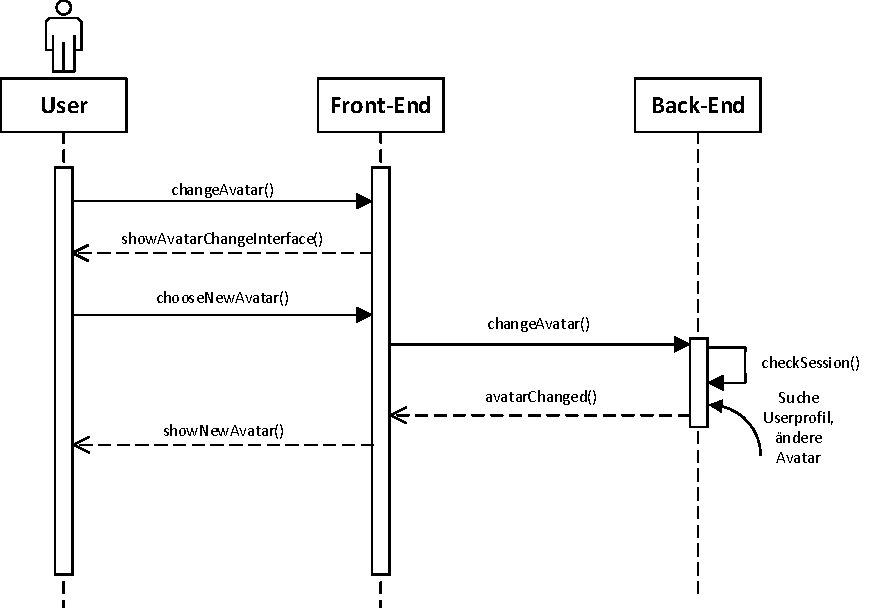
\includegraphics[width=1.3\textwidth]{figures/sequenz_F70.pdf}
\caption{Sequenzdiagramm zum Ändern des Avatars}
\label{sequence}
\end{figure}
Das Diagramm 2.6 beschreibt das Ändern des Avatars.

Klickt der User auf den Change Avatar Button, werden ihm alle seine verfügbaren Avatare angezeigt und er kann sich für einen entscheiden. Hat er dies getan wird die Änderung der Einstellung vermerkt, ans Back-End geschickt, dort gespeichert und dann, wieder zurück im Front-End, aktualisiert angezeigt.
%==================================================================

\newpage
\section{Analyse von Funktionalität <F80>: <Benutzer löschen>} 
\begin{figure}[h]
\centering
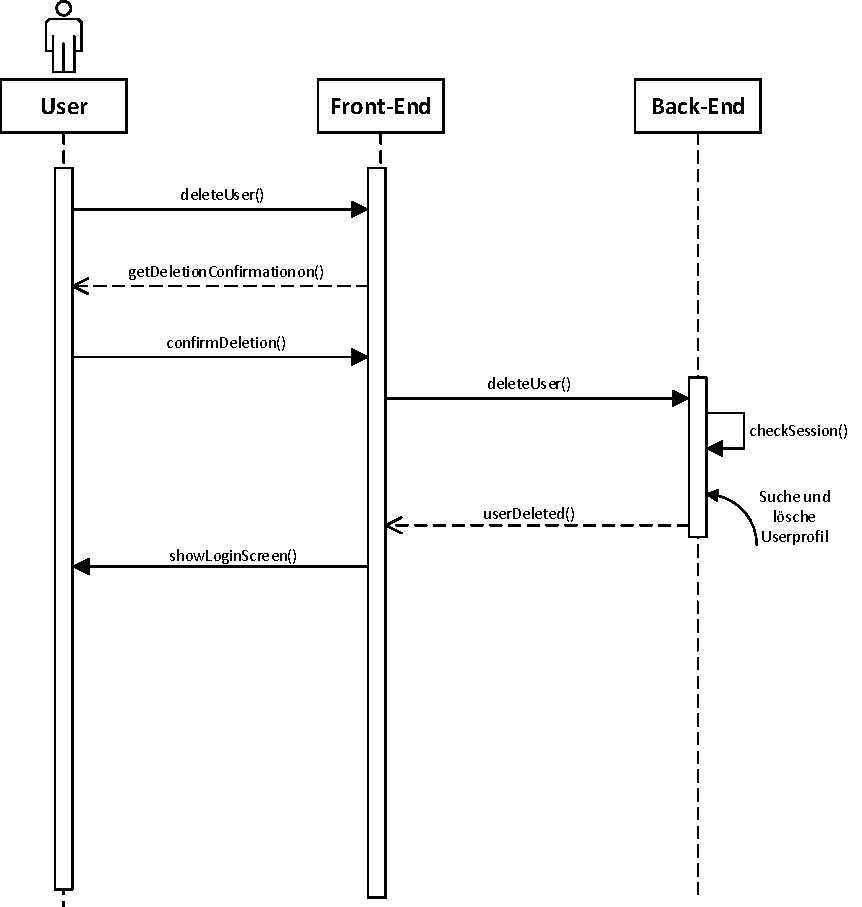
\includegraphics[width=1.3\textwidth]{figures/sequenz_F80.pdf}
\caption{Sequenzdiagramm zum Löschen des Benutzers}
\label{sequence}
\end{figure}
Diagramm 2.7 zeigt, was passiert, wenn der User seinen Account löschen möchte.

Möchte der User sein Profil löschen, kann er dies im Settings-Interface tun, was dem entsprechend erst geladen werden muss. Wenn der User nun den Delete User Button drückt, wird der User erst noch einmal gefragt, ob er ein Profil wirklich löschen möchte. Beantwortet der User dies positiv geht eine Mitteilung an das Back-End, wo das Profil gelöscht wird und der User auf den Login-Screen geleitet wird wo es ihm frei steht, sich wieder zu registrieren.
%==================================================================

\newpage
\section{Analyse von Funktionalität <F90>: <Audioeinstellungen bearbeiten>}
\begin{figure}[h]
\centering
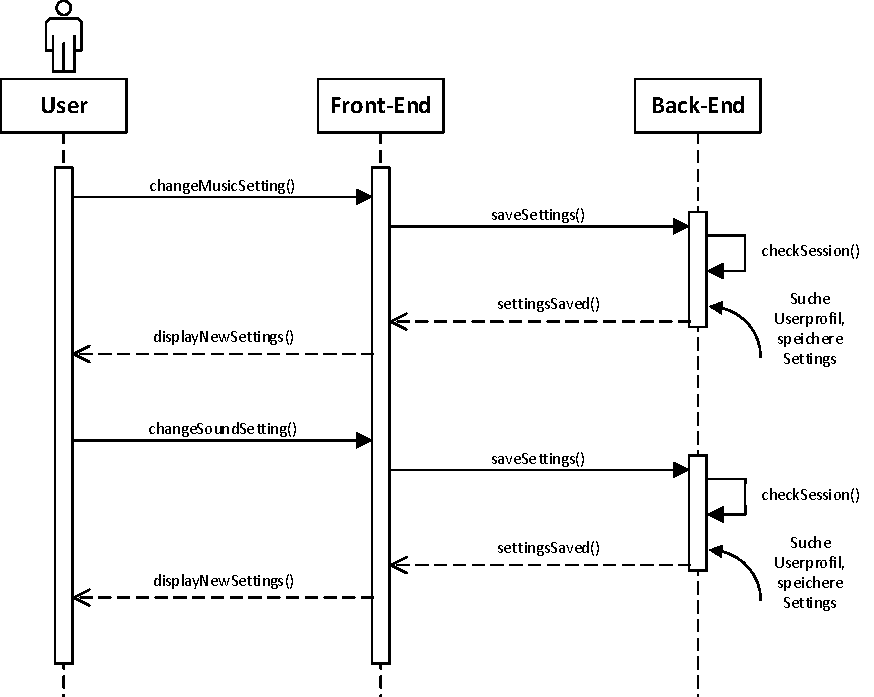
\includegraphics[width=1.3\textwidth]{figures/sequenz_F90.pdf}
\caption{Sequenzdiagramm zum Ändern der Audioeinstellungen}
\label{sequence}
\end{figure}
Diagramm 2.8 zeigt, was passiert, wenn der User seine Audio-Optionen ändert.

Zum Ändern der Audiofunktionen stehen Knöpfe bereit, die sowohl die Hintergrundmusik (\glqq Music\grqq) als auch die Soundeffekte, wie Sprungsounds und Klicksounds,  aus- beziehungsweise einstellen. Jegliche \"Anderung wird sofort ans Back-End gesendet, dort gespeichert und dann im Profil aktualisiert.
%==================================================================

\newpage
\section{Analyse von Funktionalität <F100>: <Spielstand zurücksetzen>}
\begin{figure}[h]
\centering
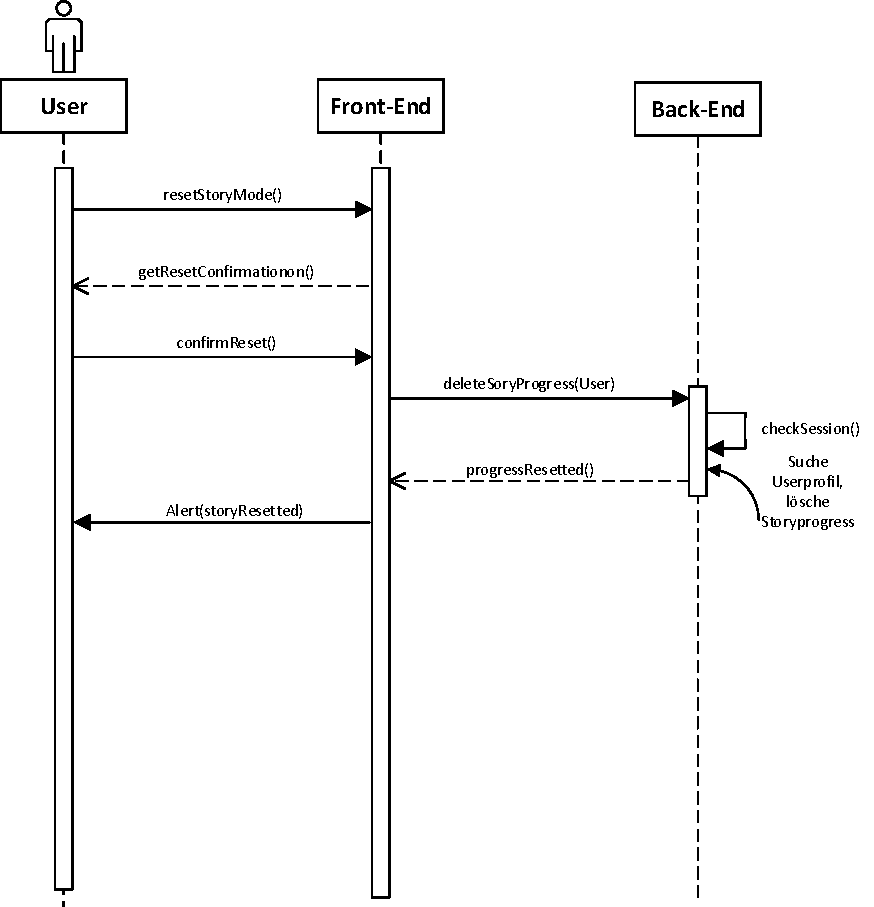
\includegraphics[width=1.3\textwidth]{figures/sequenz_F100.pdf}
\caption{Sequenzdiagramm zum Zurücksetzen des Spielstands}
\label{sequence}
\end{figure}
Diagramm 2.9 beschreibt das Zurücksetzen des Storyfortschrittes.

Der User kann per Knopfdruck seinen Story-Fortschritt zurücksetzen. Tut er dies, muss er vorher noch einmal seine Zustimmung zum Löschvorgang geben. Ist auch dies geschehen, wird die Anweisung zum Löschen des Storyfortschrittes des Users an das Back-End geschickt und dort ausgeführt.
%==================================================================

\newpage
\section{Analyse von Funktionalität <F110>: <Tutorial spielen>}
\begin{figure}[h]
\centering
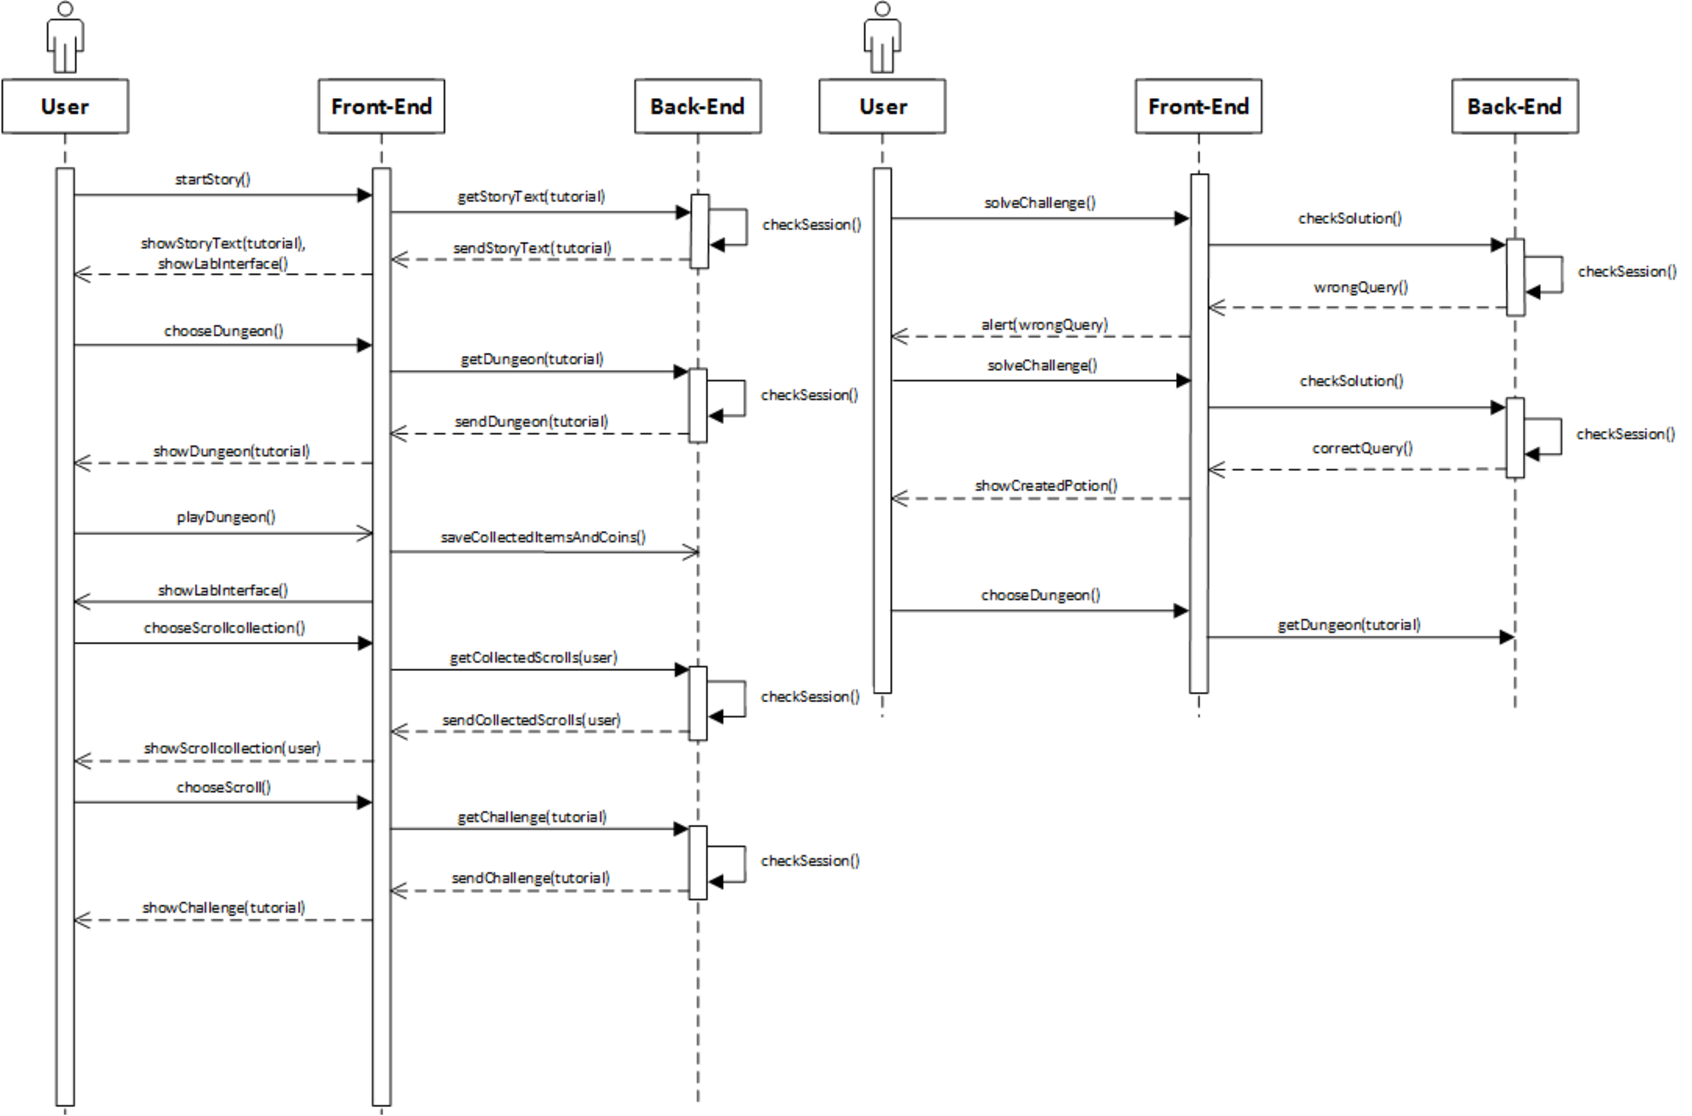
\includegraphics[width=1.0\textwidth]{figures/sequenz_F110.pdf}
\caption{Sequenzdiagramm für das Tutorial}
\label{sequence}
\end{figure}
Diagramm 2.10 zeigt den Ablauf im Tutorial.

Wird das Tutorial gestartet, werden zuerst alle Tutorial-Texte vom Back-End angefordert. Diese werden dann, wenn benötigt, dem User angezeigt. Zuerst wird der User in den Dungeon geleitet. Dafür werden die Leveldaten vom Back-End geladen, sodass der User den Dungeon betreten und Spielen kann. Hierbei kann er Schriftrollen (\glqq Scrolls\grqq) und Münzen (\glqq Lofi-Coins\grqq) einsammeln, was jeweils sofort ans Back-End gesendet und dort im Story-Progress bzw. in den Profildaten gespeichert wird.
Scheitert der User an einer Hürde im Dungeon, bekommt er zuerst einen Game-Over-Screen angezeigt, auf dem zusehen ist, was er eingesammelt hat und wird zur\"uck in den Labor-Screen geleitet.
Dort wird er per Tutorial-Text zur Scrollcollection geleitet um sich dort für ein Trank-Rezept zu entscheiden. Ist dies getan, wird aus dem Back-Ende eine für das Rezept passende Aufgabe angefordert und dem User angezeigt. Für diese Aufgabe hat der User keine Versuchsbegrenzung. Die Eingaben des Users werden dabei immer an das Back-End gesendet und dort kontrolliert. Hat der User die Aufgabe richtig gelöst, erhält er eine Potion und kann diese danach im Dungeon verwenden.
%==================================================================

\newpage
\section{Analyse von Funktionalität <F120>: <Story spielen>}
\begin{figure}[h]
\centering
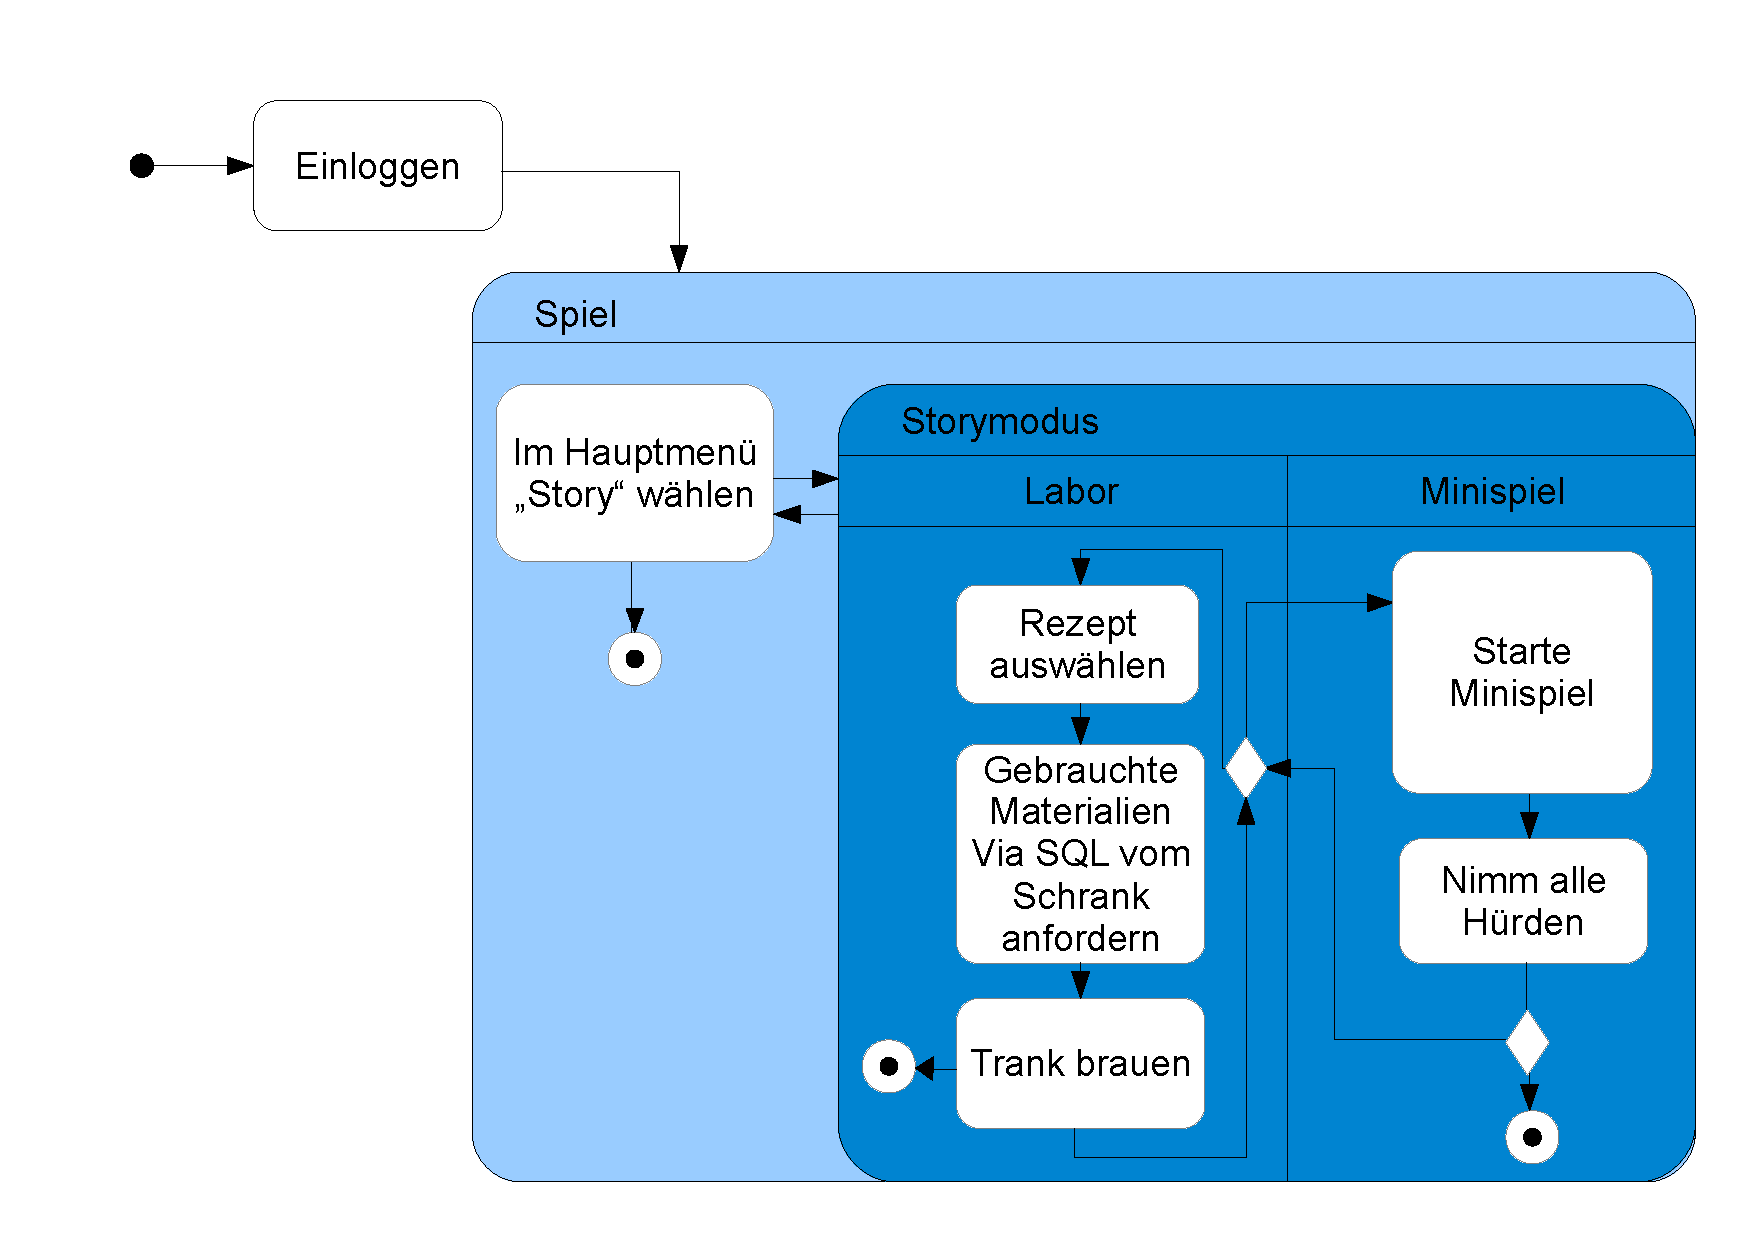
\includegraphics[width=1.0\textwidth]{figures/Aktivitaetsdiagramm.pdf}
\caption{Aktivitätsdiagramm für den Story Mode}
\label{sequence}
\end{figure}
Der Story-Mode besteht aus sich abwechselnden Teilen aus SQL-Trainer und Minispiel. Um dies  besser zu zeigen, ist in Abbildung 2.11  das Aktivitätsdiagramm für den Story Mode aus dem Pflichtenheft abgebildet.

Darin ist zusehen, dass man sich im Labor einen oder mehrere Tränke brauen kann (SQL-Trainer-Anteil) um diese dann im Dungeon zu verwenden (Minispiel-Anteil).
Um die beiden Teile für sich besser beschreiben zu können, sind diese in den folgenden zwei Funktionen aufgeführt.
%==================================================================

\newpage
\section{Analyse von Funktionalität <F130>: <SQL-Trainer spielen>}
\begin{figure}[h]
\centering
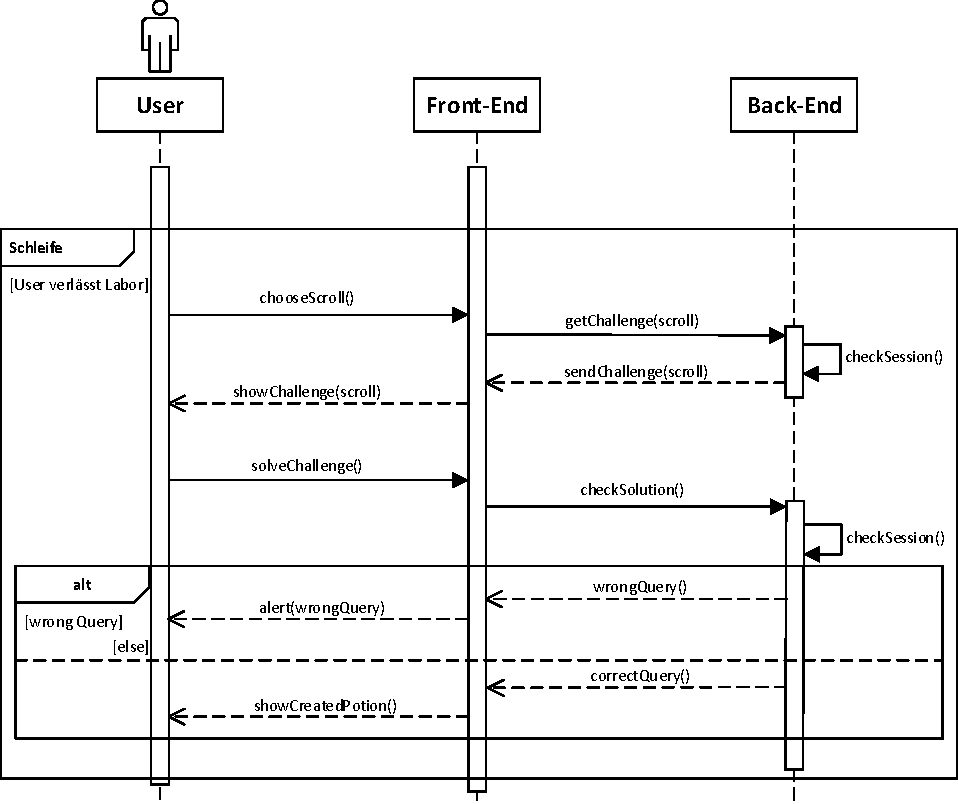
\includegraphics[width=1.3\textwidth]{figures/sequenz_F130.pdf}
\caption{Sequenzdiagramm für den SQL-Trainer}
\label{sequence}
\end{figure}


Der SQL-Trainer ist Teil der drei Spielmodi (Story, Trivia, Homework) und wird einmal, wie er im Trivia-Mode verwendet wird, erklärt. Die leichten Abweichungen der anderen Spielmodi werden im Anschluss erwähnt. Diese benötigen wenig bis gar keine weitere Erklärung, da sie nur einen oberflächlichen Unterschied machen.

Zuerst werden dem User f\"unf Schwierigkeitsgrade angezeigt aus denen der er wählen kann. Hat er sich für einen Schwierigkeitsgrad entschieden, wird dies dem Back-End mitgeteilt, was daraufhin eine, dem gewählten Schwierigkeitsgrad entsprechende, Aufgabe bereitstellt. Diese kann dann vom User gelöst werden. Die Eingaben werden dabei immer ans Back-End geschickt und dort auf Richtigkeit geprüft. 

Ist die Prüfung positiv verlaufen wird der User wieder zur Schwierigkeitsgrad-Auswahl weitergeleitet.


Abweichungen zum Story-Mode:\\
Es werden keine Schwierigkeitsgrade angezeigt, sondern schon eingesammelte Rezepte für Tränke. Diese beinhalten in ihrer Definition schon die Schwierigkeitsgrade für die daraus hervorgehenden Aufgaben.


Abweichungen zum Homework-Mode:\\
Beim Homework-Mode wird die Auswahl des Schwierigkeitsgrades in jeglicher Form übersprungen und der Aufgabentext wird direkt angezeigt.  
%==================================================================

\newpage
\section{Analyse von Funktionalität <F140>: <Minispiel spielen>}
\begin{figure}[h]
\centering
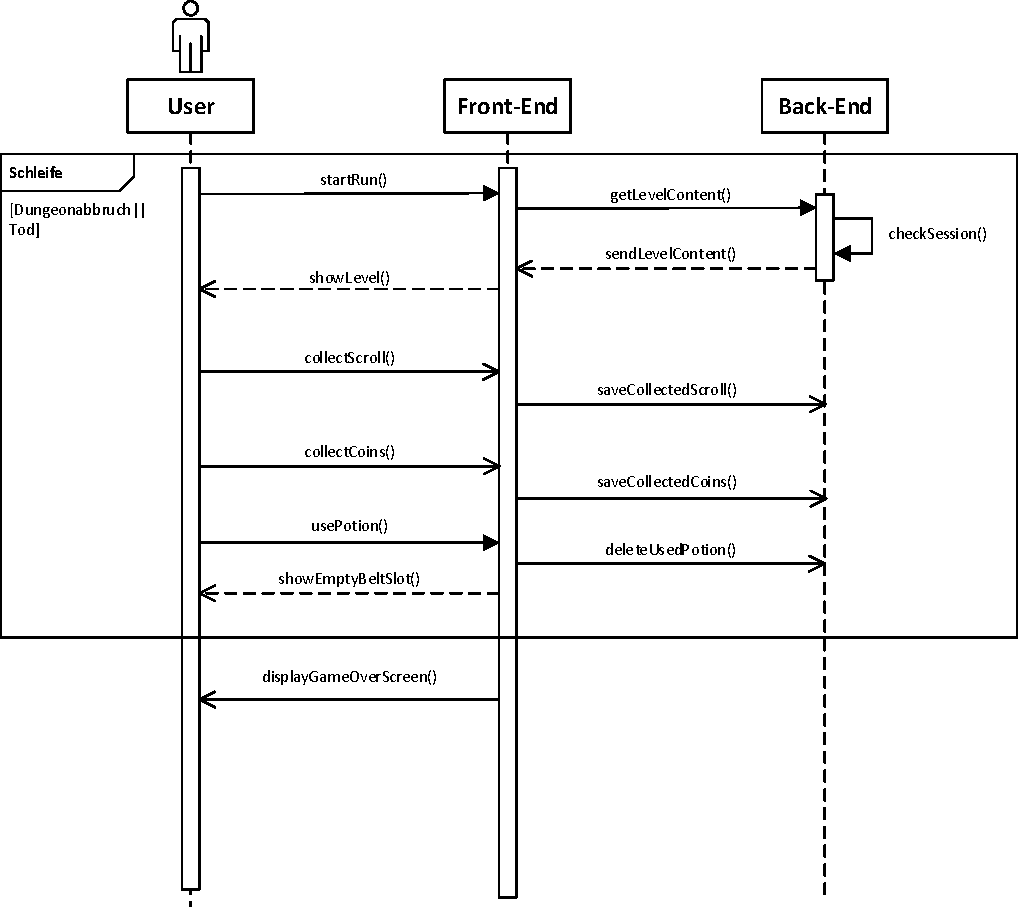
\includegraphics[width=1.3\textwidth]{figures/sequenz_F140.pdf}
\caption{Sequenzdiagramm für das Minigame}
\label{sequence}
\end{figure}
Die Abbildung 2.13 zeigt die Abläufe im Dungeon.

Im Minispiel bewegt sich die Figur stetig nach rechts. Der User kann springen, wodurch er verschiedene Hindernisse überwinden kann. Desweiteren kann der User Lofi-Coins und Scrolls einsammeln. Dies wird sofort im Back-End vermerkt und im Spielerprofil und im Storyprogress gespeichert. Dem User ist zudem möglich vorher erstellte Potions zu verwenden um deren Effekte zur Überwindung von Hindernissen zu nutzen.

%==================================================================

\section{Analyse von Funktionalität <F150>: <Hausaufgaben bearbeiten>}
Die Bearbeitung von Hausaufgaben funktioniert wie das Nutzen des SQL-Trainers. Genauere Erklärungen sind dort (F130) zufinden.
%==================================================================

\section{Analyse von Funktionalität <F160>: <Ranglisten einsehen>}
\begin{figure}[h]
\centering
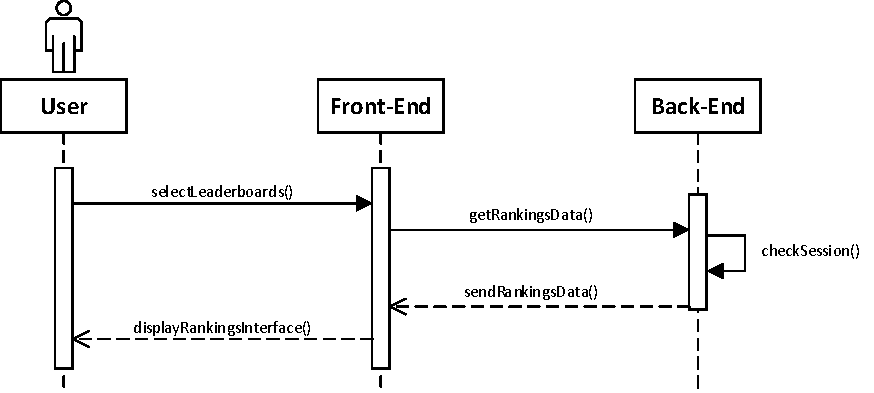
\includegraphics[width=1.2\textwidth]{figures/sequenz_F160.pdf}
\caption{Sequenzdiagramm für die Ranglisten}
\label{sequence}
\end{figure}
In Abbildung 2.14 wir das Anzeigen der Ranglisten dargestellt.

Möchte der User die Ranglisten einsehen, wird eine Anfrage an das Back-End gesendet. Das Back-End stellt dann die Daten für die Ranglisten zusammen und sendet diese dann zurück ans Front-End wo diese dann für den User einsehbar präsentiert werden.
%==================================================================

\newpage
\section{Analyse von Funktionalität <F170>: <Spieler suchen>}
\begin{figure}[h]
\centering
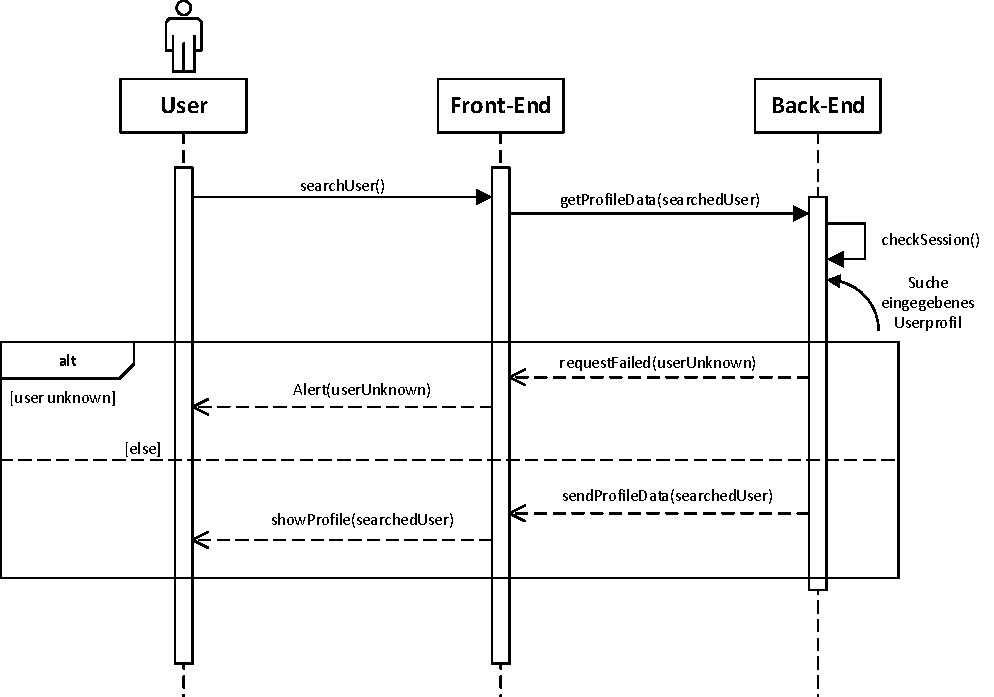
\includegraphics[width=1.3\textwidth]{figures/sequenz_F170.pdf}
\caption{Sequenzdiagramm zum Suchen eines anderen Users}
\label{sequence}
\end{figure}
Im Diagramm 2.15 ist zu sehen, wie man nach einem anderen User suchen kann.

Um einen anderen User zu suchen wird ein Usersuche-Feld bereitgestellt. Der dort eingegebene Name wird an das Back-End weitergeleitet und dort in der Userdatenbank gesucht und wenn er existiert wird dessen Profil aus der Datenbank geladen dem suchenden User angezeigt. Ist der Name in der Datenbank nicht zu finden, wird dem suchenden User das mitgeteilt.
%================================================================== 

\newpage
\section{Analyse von Funktionalität <F180>: <Hausaufgabenergebnisse einsehen>}
\begin{figure}[h]
\centering
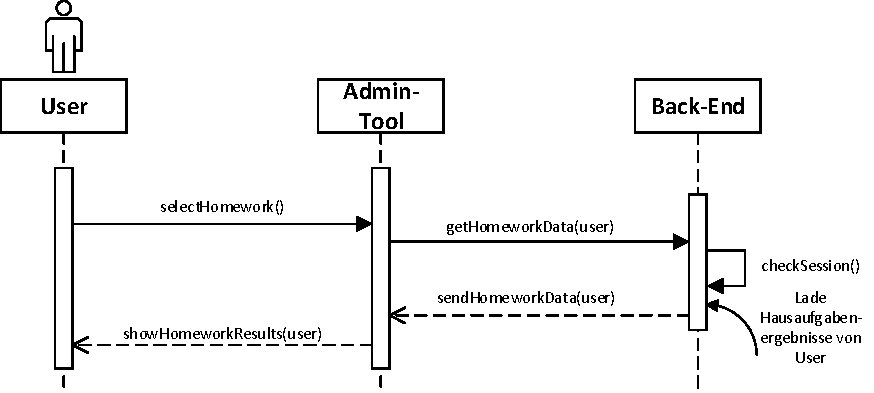
\includegraphics[width=1.3\textwidth]{figures/sequenz_F180.pdf}
\caption{Sequenzdiagramm zum einsehen der eigenen Hausaufgabenergebnisse}
\label{sequence}
\end{figure}
Abbildung 2.16 beschreibt das Anzeige der Hausaufgabenergebnisse.

Nach dem Einloggen in das Admintool werden die Hausaufgabenergebnisse eines nicht-beförderten Users direkt aus der Datenbank geladen und angezeigt.
Ist der User schon \glqq befördert\grqq muss er erst noch auf den Show Homework Results Button drücken.
%==================================================================

\newpage
\section{Analyse von Funktionalität <F190>: <Benutzer befördern>}
\begin{figure}[h]
\centering
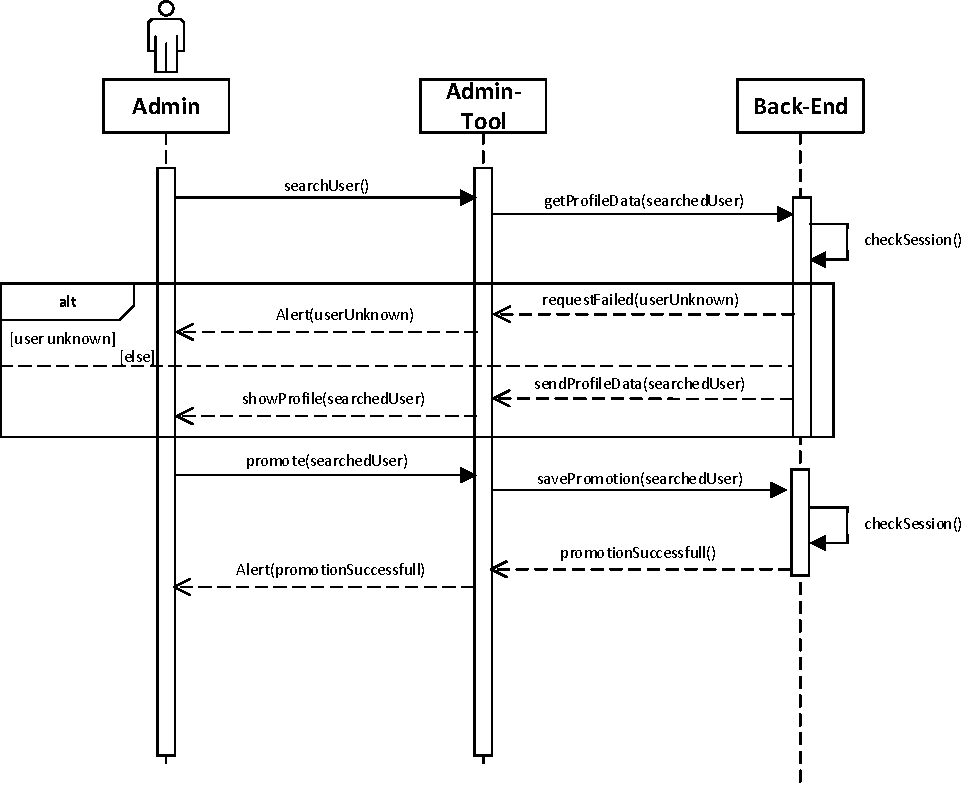
\includegraphics[width=1.3\textwidth]{figures/sequenz_F190.pdf}
\caption{Sequenzdiagramm zum Befördern eines Users}
\label{sequence}
\end{figure}
Abbildung 2.17 beschreibt das Befördern eines Benutzers.

Zuerst wird für den Admin die Userdatenbank angzeigt. Hier kann er entweder manuell oder per Suchfunktion nach einem User suchen und per Knopfdruck befördern, was dann im Back-End in den jeweiligen Userdaten registriert und gespeichert wird. 

Der Ablauf, einen User Adminrechte (<F200>) zu geben, gleicht dem des User Bef\"orderns.
%==================================================================

\newpage
\section{Analyse von Funktionalität <F210>: <Eine Trivia-Aufgabe erstellen>}
\begin{figure}[h]
\centering
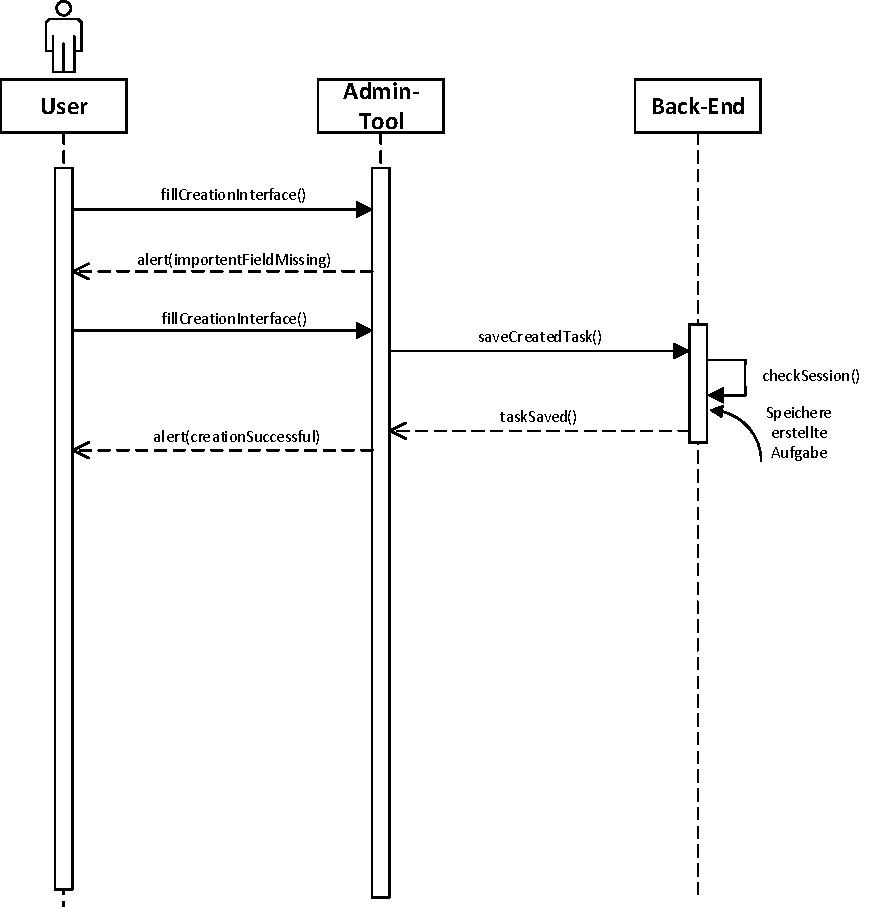
\includegraphics[width=1.3\textwidth]{figures/sequenz_F210.pdf}
\caption{Sequenzdiagramm für das Erstellen von Aufgaben}
\label{sequence}
\end{figure}
Abbildung 2.18 beschreibt das Erstellen von eigenen Aufgaben.

Beförderte Nutzer können selber Aufgaben erstellen die später im Trivia Mode verwendet werden können.
Dafür steht im Admin-Tool ein Interface zur Verfügung in das ganz einfach alle zur Aufgabe gehörigen Daten einsammelt und dann ans Back-End sendet, welches die Aufgabe dann speichert. Sind nicht alle wichtigen Felder ausgefüllt, wird der User alarmiert und muss dies berichtigen damit dich Aufgabe gespeichert werden kann.
%==================================================================

\newpage
\section{Analyse von Funktionalität <F220>: <Benutzeraufgaben bewerten>}
\begin{figure}[h]
\centering
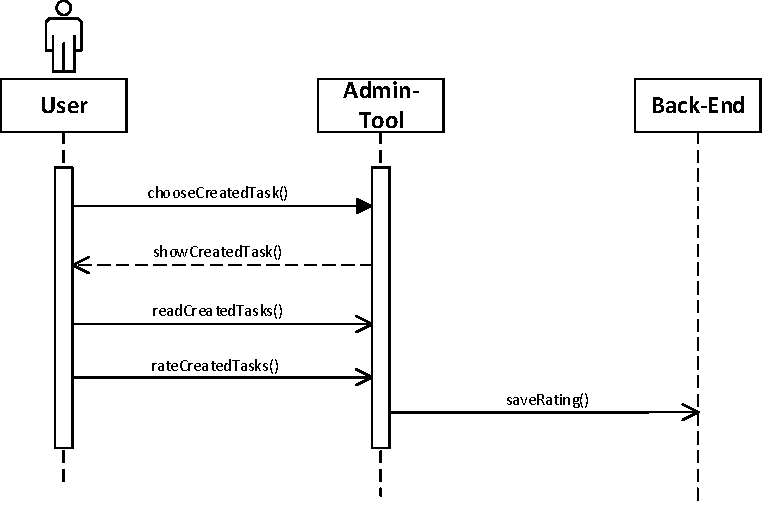
\includegraphics[width=1.3\textwidth]{figures/sequenz_F220.pdf}
\caption{Sequenzdiagramm zum bewerten User-erstellter Aufgaben.}
\label{sequence}
\end{figure}
Abbildung 2.19 zeigt den Ablauf, wie man eine User-erstellte Aufgabe bewertet.

In der Liste aller User-erstellten Aufgaben kann sich der User Aufgaben aussuchen, diese Ansehen und sie bewerten und kommentieren. Die Bewertung wird dann im Back-End für die Aufgabe registriert und gespeichert. 
%==================================================================

\newpage
\section{Analyse von Funktionalität <F230>: <Hausaufgaben erstellen>}

Die Erstellung von Hausaufgaben gleicht der User-seitigen Erstellung von Aufgaben, ist jedoch nur Administratoren zugänglich.

Der Unterschied zur normalen Aufgabenerstellung besteht darin, dass ein Aufgabenpaket erstellt wird. Dabei kann man entweder Aufgaben für das Paket neu erstellen, oder auf schon einmal erstellte Aufgaben, die in der Datenbank gespeichert sind, zugreifen. Diese Aufgabenpakete können dann noch mit zusätzlichen Parametern versehen werden, wie zum Beispiel einem Bearbeitungszeitraum oder einer Anzahl an Versuchen. 

%!TEX root = ../Fachentwurf.tex

\chapter{Datenmodell}

Das folgende Kapitel beschreibt die Datensätze, welche der SQL-Alchemist dauerhaft oder teilweise auch nur temporär abspeichert.
Dazu werden zuerst einige Erl\"auterungen zu den einzelnen Beziehungen angegeben und zum Ende des Kapitels ist ein Klassen-Diagramm zur Veranschaulichung dieses Sachverhaltes abgebildet.


\section{Erläuterung}


\begin{entity}{10}{Avatar}
\begin{center}
	\begin{longtable}{|m{4cm}|m{2,5cm}|m{4,5cm}|m{3,5cm}|}
 	 \hline
 	 \textbf{Beziehung} & \textbf{Kardinalität} &  \textbf{Erwartete Datenmenge} & \textbf{Beschreibung} \\
  	\hline
  	Profile & 0 ... *   & Min: <...>, Max: <...> & Der Avatar wird vom Profil als Erkennungsmerkmal und Spielfigur verwendet.\\
  	  	\hline
  	Profile\_Avatar & 0 ... *   & Min: <...>, Max: <...> & Verweis auf alle vom Nutzer gekauften Avatare.\\
	  \hline
	\end{longtable}
\end{center}
Die Entitäten vom Typ \glqq Avatar\grqq~beschreiben die verschiedenen vom Spiel zur Verfügung gestellten Spielfiguren. Diese werden sowohl im Minispiel als auch als Erkennungsmerkmal der Profile der Nutzer verwendet.
In der Datenbank werden unter anderem die zugehörigen Eigenschaften, sowie die Darstellungsmerkmale gespeichert.
\textbf{Hinweis:} In der Relation Profile\_Avatar sind die Avatare mit den Profilen verknüpft, das Profil verfügt jedoch zusätzlich über das Attribut "Avatar". Der im Profil gespeicherte Avatar ist dabei der aktuell verwendete.
\end{entity}


\newpage
\begin{entity}{20}{Bag\_Slot}
\begin{center}
	\begin{longtable}{|m{4cm}|m{2,5cm}|m{4,5cm}|m{3,5cm}|}
 	 \hline
 	 \textbf{Beziehung} & \textbf{Kardinalität} &  \textbf{Erwartete Datenmenge} & \textbf{Beschreibung} \\
  	\hline
  	Potion & 1  & Min: <...>, Max: <...> & In Bagslots werden die bereits gesammelten Tränke gespeichert.\\
	  \hline
  	Profile & 1  & Min: <...>, Max: <...> & Ein Bagslot gehört einem Profil.\\
	  \hline
	\end{longtable}
\end{center}
Bei den Entitäten des Typs \glqq Bag\_Slot\grqq~handelt es sich um die einzelnen Plätze innerhalb des Inventars der Nutzer, in denen alle hergestellten Tränke abgelegt werden. Dabei nimmt jeder Slot genau einen Trank auf. \\\\\
\end{entity}


\begin{entity}{30}{Challenge}
\begin{center}
	\begin{longtable}{|m{4cm}|m{2,5cm}|m{4,5cm}|m{3,5cm}|}
 	 \hline
 	 \textbf{Beziehung} & \textbf{Kardinalität} &  \textbf{Erwartete Datenmenge} & \textbf{Beschreibung} \\
  	\hline
  	Map\_In\_Challenge & 0 ... *  & Min: <...>, Max: <...> & Eine Challenge kann mit mehreren Maps verknüpft sein.\\
  	\hline
  	Solve\_Challenge & 0 ... *  & Min: <...>, Max: <...> & Bearbeitungsfortschritt der Challenge, verknüpft mit dem Profil\\
	  \hline
  	Text\_In\_Challenge & 0 ... *  & Min: <...>, Max: <...> & Story-Texte können Challenges zugeordnet werden, um diese in den Kontext der Handlung einzubinden. \\
	  \hline
	Task\_In\_Challenge & 1 ... * & Min: <...>, Max: <...> & Eine Challenge besteht aus mindestens einer Aufgabe.\\
	  \hline
	\end{longtable}
\end{center}
Die \glqq Challenge\grqq-Objekte beschreiben die Aufgabenpakete, welche zum Beispiel im Laufe der Story oder als Hausaufgaben an die Nutzer gestellt werden. Jedes dieser Pakete besteht aus verschiedenen Aufgaben. Als Attribute werden alle Informationen, die zur Beschreibung eines solchen Paketes benötigt werden in der Datenbank gespeichert.\\\\\\\
\end{entity}

\begin{entity}{40}{Map}
\begin{center}
	\begin{longtable}{|m{4cm}|m{2,5cm}|m{4,5cm}|m{3,5cm}|}
 	 \hline
 	 \textbf{Beziehung} & \textbf{Kardinalität} &  \textbf{Erwartete Datenmenge} & \textbf{Beschreibung} \\
  	\hline
  	Map\_In\_Challenge & 0 ... *   & Min: <...>, Max: <...> & Eine Map kann in mehreren Challenges verwendet werden.\\
	  \hline
	\end{longtable}
\end{center}
Bei den \glqq Map\grqq-Entitäten handelt es sich um die verschiedenen Levels, aus denen das Minispiel besteht. \\\\\\\
\end{entity}

\begin{entity}{50}{Map\_In\_Challenge}
\begin{center}
	\begin{longtable}{|m{4cm}|m{2,5cm}|m{4,5cm}|m{3,5cm}|}
 	 \hline
 	 \textbf{Beziehung} & \textbf{Kardinalität} &  \textbf{Erwartete Datenmenge} & \textbf{Beschreibung} \\
  	\hline
  	Challenge & 1  & Min: <...>, Max: <...> & Verweis auf die Challenge\\
	  \hline
  	Map & 1  & Min: <...>, Max: <...> & Verweis auf die Map\\
	  \hline
	\end{longtable}
\end{center}
In diesen Objekten werden die Beziehungen der \glqq Maps\grqq~und der \glqq Challenges\grqq~festgehalten. Dies umfasst, welche Level des Minispiels für die Lösung bestimmter Aufgabenpakete abgeschlossen werden müssen und in welcher Reihenfolge diese auftreten. \\\
\end{entity}

\begin{entity}{60}{Potion}
\begin{center}
	\begin{longtable}{|m{4cm}|m{2,5cm}|m{4,5cm}|m{3,5cm}|}
 	 \hline
 	 \textbf{Beziehung} & \textbf{Kardinalität} &  \textbf{Erwartete Datenmenge} & \textbf{Beschreibung} \\
  	\hline
  	Bag\_Slot & 0 ... *  & Min: <...>, Max: <...> & Die Potion wird in einem Bagslot abgelegt.\\
	  \hline
  	Scroll & 1  & Min: <...>, Max: <...> & Die Potion ist einer Scroll zugeordnet. \\
	  \hline
  	Task & 1 ... *  & Min: <...>, Max: <...> & Zum Erzeugen der Potion muss eine Aufgabe gelöst werden.\\
	  \hline
	\end{longtable}
\end{center}
Die \glqq Potion\grqq-Entitäten beschreiben die Tränke, welche die Spieler im Laufe des Spiels herstellen. Dazu werden die Auswirkungen der Tränke als Attribute gespeichert. \\\\\\\
\end{entity}

\begin{entity}{70}{Profile}
\begin{center}
	\begin{longtable}{|m{4cm}|m{2,5cm}|m{4,5cm}|m{3,5cm}|}
 	 \hline
 	 \textbf{Beziehung} & \textbf{Kardinalität} &  \textbf{Erwartete Datenmenge} & \textbf{Beschreibung} \\
  	\hline
  			Avatar & 1 & Min: <...>, Max: <...> & Jedes Profil besitzt einen Avatar, der dieses repräsentiert.\\
	  \hline
	    	Bag\_Slot & 0 ... * & Min: <...>, Max: <...> & Bagslots, die dem Profil gehören.\\
	  \hline
  			Profile\_Avatar & 1 ... *  & Min: <...>, Max: <...> & Dem Profil zur Verfügung stehende Avatare.\\
	  \hline
	    	Comment\_Task & 0 ... * & Min: <...>, Max: <...> & In dieser Relation wird auf die vom Nutzer kommentierten Aufgaben verwiesen. \\
	  \hline
	    	Rate\_Task & 0 ... * & Min: <...>, Max: <...> & In dieser Relation wird auf die vom Nutzer bewerteten Aufgaben verwiesen.\\
	  \hline
	    	Profile\_Scroll & 0 ... * & Min: <...>, Max: <...> & Das Profil sammelt Schriftrollen in der Scrollcollection.\\
	  \hline
	    	Profile\_Shop\_Item & 0 ... * & Min: <...>, Max: <...> & Relation mit gekauften Items im Shop.\\
	  \hline
			Solve\_Challenge & 0 ... * & Min: <...>, Max: <...> & Challenges, zu denen der Nutzer Zugang hat.\\
	  \hline 
	    	Solve\_Task & 0 ... * & Min: <...>, Max: <...> & Tasks, zu denen der Nutzer Zugang hat.\\
	  \hline
  	  		User & 1  & Min: <...>, Max: <...> &  Jedes Profil gehört einem Nutzer.\\
	  \hline
	\end{longtable}
\end{center}
Die Entitäten des Typs \glqq Profile\grqq~stellen die zentrale Verwaltungsstelle der Nutzer dar. Über diese wird der Fortschritt der Spieler abgewickelt, deren Einstellungen gespeichert und die Eigenschaften der Spielfiguren festgehalten. 
\end{entity}

\newpage
\begin{entity}{80}{Profile\_Avatar}
\begin{center}
	\begin{longtable}{|m{4cm}|m{2,5cm}|m{4,5cm}|m{3,5cm}|}
 	 \hline
 	 \textbf{Beziehung} & \textbf{Kardinalität} &  \textbf{Erwartete Datenmenge} & \textbf{Beschreibung} \\
  	\hline
	Avatar & 1  & Min: <...>, Max: <...> & Verweis auf ein Avatar\\
	  \hline
  	Profile & 1  & Min: <...>, Max: <...> & Verweis auf ein Profil\\
	  \hline
	\end{longtable}
\end{center}
Diese Entitäten halten die durch ein Profil gekauften Avatare fest und speichert dazu wann die Transaktion durchgeführt wurde.\\\\\\\
\end{entity}

\begin{entity}{90}{Comment\_Task}
\begin{center}
	\begin{longtable}{|m{4cm}|m{2,5cm}|m{4,5cm}|m{3,5cm}|}
 	 \hline
 	 \textbf{Beziehung} & \textbf{Kardinalität} &  \textbf{Erwartete Datenmenge} & \textbf{Beschreibung} \\
  	\hline
	Profile & 1  & Min: <...>, Max: <...> & Verweis auf das Profil\\
	  \hline
  	Task & 1  & Min: <...>, Max: <...> & Verweis auf die Aufgabe\\
	  \hline
	\end{longtable}
\end{center}
Über die \glqq Comment\_Task\grqq-Objekte werden die durch die Nutzer kommentierten Aufgaben gespeichert. Als Attribut wird dazu unter anderem das jeweilige Kommentar festgehalten.\\\\\\\
\end{entity}

\begin{entity}{100}{Rate\_Task}
\begin{center}
	\begin{longtable}{|m{4cm}|m{2,5cm}|m{4,5cm}|m{3,5cm}|}
 	 \hline
 	 \textbf{Beziehung} & \textbf{Kardinalität} &  \textbf{Erwartete Datenmenge} & \textbf{Beschreibung} \\
  	\hline
	Profile & 1  & Min: <...>, Max: <...> & Verweis auf das Profil\\
	  \hline
  	Task & 1  & Min: <...>, Max: <...> & Verweis auf die Aufgabe\\
	  \hline
	\end{longtable}
\end{center}
Über die \glqq Rate\_Task\grqq-Objekte werden die durch die Nutzer bewerteten Aufgaben gespeichert. Als Attribut wird dazu unter anderem die jeweilige Bewertung festgehalten.\\\\\\\
\end{entity}

\begin{entity}{110}{Profile\_Scroll}
\begin{center}
	\begin{longtable}{|m{4cm}|m{2,5cm}|m{4,5cm}|m{3,5cm}|}
 	 \hline
 	 \textbf{Beziehung} & \textbf{Kardinalität} &  \textbf{Erwartete Datenmenge} & \textbf{Beschreibung} \\
  	\hline
	Profile & 1  & Min: <...>, Max: <...> & Verweis auf das Profil\\
	  \hline
  	Scroll & 1  & Min: <...>, Max: <...> & Verweis auf die Scroll\\
	  \hline
	\end{longtable}
\end{center}
Hier werden die von den Nutzern gesammelten Scrolls gespeichert.\\\\\\\
\end{entity}

\begin{entity}{120}{Profile\_Shop\_Item}
\begin{center}
	\begin{longtable}{|m{4cm}|m{2,5cm}|m{4,5cm}|m{3,5cm}|}
 	 \hline
 	 \textbf{Beziehung} & \textbf{Kardinalität} &  \textbf{Erwartete Datenmenge} & \textbf{Beschreibung} \\
  	\hline
	Profile & 1  & Min: <...>, Max: <...> & Verweis auf das Profil\\
	  \hline
  	Shop\_Item & 1  & Min: <...>, Max: <...> & Verweis auf das Shop-Item\\
	  \hline
	\end{longtable}
\end{center}
Die Entitäten des Typs \glqq Profile\_Shop\_Item\grqq~halten fest, welche Spielgegenstände die Spieler bisher bereits erworben haben.
\end{entity}

\newpage
\begin{entity}{130}{Solve\_Challenge}
\begin{center}
	\begin{longtable}{|m{4cm}|m{2,5cm}|m{4,5cm}|m{3,5cm}|}
 	 \hline
 	 \textbf{Beziehung} & \textbf{Kardinalität} &  \textbf{Erwartete Datenmenge} & \textbf{Beschreibung} \\
  	\hline
  	Challenge & 1  & Min: <...>, Max: <...> & Verweis auf die Challenge\\
	  \hline
	Profile & 1  & Min: <...>, Max: <...> & Verweis auf das Profil\\
	  \hline
	\end{longtable}
\end{center}
Diese Objekte halten den Bearbeitungsfortschritt der Nutzer bezüglich der Aufgabenpakete fest. Es werden dabei sowohl die bereits gelösten Aufgabenpakete, als auch die noch nicht abgeschlossenen Aufgabenpakete abgespeichert.\\\\\\\
\end{entity}

\begin{entity}{140}{Solve\_Task}
\begin{center}
	\begin{longtable}{|m{4cm}|m{2,5cm}|m{4,5cm}|m{3,5cm}|}
 	 \hline
 	 \textbf{Beziehung} & \textbf{Kardinalität} &  \textbf{Erwartete Datenmenge} & \textbf{Beschreibung} \\
  	\hline
	Profile & 1  & Min: <...>, Max: <...> &  Verweis auf das Profil\\
	  \hline
  	Task & 1  & Min: <...>, Max: <...> & Verweis auf die Aufgabe.\\
	  \hline
	\end{longtable}
\end{center}
Diese Entitäten sorgen für die Speicherung des Fortschritts bei der Lösung der einzelnen Aufgaben durch die verschiedenen Nutzer. Dabei werden unter anderem die benötigte Zeit, sowie das Lösungsdatum als Attribute gespeichert.
\end{entity}

\newpage
\begin{entity}{150}{Scroll}
\begin{center}
	\begin{longtable}{|m{4cm}|m{2,5cm}|m{4,5cm}|m{3,5cm}|}
 	 \hline
 	 \textbf{Beziehung} & \textbf{Kardinalität} &  \textbf{Erwartete Datenmenge} & \textbf{Beschreibung} \\
  	\hline
  	Potion & 0 .. 1  & Min: <...>, Max: <...> & Jede Schriftrolle schaltet eine oder keine Potion frei.\\
	  \hline
	Profile\_Scroll & 0 ... * & Min: <...>, Max: <...> & Eine gesammelte Schriftrolle wird in der Scrollcollection des Profils gespeichert.\\
	  \hline
	\end{longtable}
\end{center}
Die \glqq Scrolls\grqq~beschreiben die im Spiel verteilten Schriftrollen, welche durch die Spieler eingesammelt werden um neue Tränke oder temporäre Verbesserungen der Eigenschaften der Spielfigur (Buffs) freischalten. 
\textbf{Hinweis:} Wird durch die Scroll keine Potion freigeschaltet, erhält der Nutzer einen Buff. \\\\\\\
\end{entity}

\begin{entity}{160}{Shop\_Item}
\begin{center}
	\begin{longtable}{|m{4cm}|m{2,5cm}|m{4,5cm}|m{3,5cm}|}
 	 \hline
 	 \textbf{Beziehung} & \textbf{Kardinalität} &  \textbf{Erwartete Datenmenge} & \textbf{Beschreibung} \\
  	\hline
  	Profile\_Shop\_item & 0 ... *  & Min: <...>, Max: <...> & Relation zwischen Shop-Items und den Profilen der Nutzer, die das Shop-Item gekauft haben.\\
	  \hline
	\end{longtable}
\end{center}
Die Objekte des Typs \glqq Shop\_Item\grqq~stellen die im Shop zum Kauf zur Verfügung stehenden Gegenstände dar. Daher wird unter anderem der Kaufpreis als Attribut gespeichert.
\end{entity}

\newpage
\begin{entity}{170}{Story\_Text}
\begin{center}
	\begin{longtable}{|m{4cm}|m{2,5cm}|m{4,5cm}|m{3,5cm}|}
 	 \hline
 	 \textbf{Beziehung} & \textbf{Kardinalität} &  \textbf{Erwartete Datenmenge} & \textbf{Beschreibung} \\
  	\hline
  	Text\_In\_Challenge & 1 ... * & Min: <...>, Max: <...> & Story-Texte beschreiben Challenges handlungsbezogen.\\
  	\hline
  	Text & 0 ... * & Min: <...>, Max: <...> & Texte beschreiben die Spielsituation.\\
	  \hline
	\end{longtable}
\end{center}
Diese Entitäten beschreiben die verschiedenen Texte, welche in der Story aufgerufen werden. Dazu werden die Bedingungen, welche erfüllt sein müssen um den Text aufzurufen, sowie die Reihenfolge, in der diese auftreten und deren Inhalt abgespeichert. \\\\\\\
\end{entity}

\begin{entity}{180}{Text\_In\_Challenge}
\begin{center}
	\begin{longtable}{|m{4cm}|m{2,5cm}|m{4,5cm}|m{3,5cm}|}
 	 \hline
 	 \textbf{Beziehung} & \textbf{Kardinalität} &  \textbf{Erwartete Datenmenge} & \textbf{Beschreibung} \\
  	\hline
  	Challenge & 1 & Min: <...>, Max: <...> & Verweis auf die Challenge.\\
	  \hline
	Story\_Text & 1 & Min: <...>, Max: <...> & Verweis auf den Story-Text.\\
	  \hline
	\end{longtable}
\end{center}
An dieser Stelle wird festgehalten, welche Texte in welchem Aufgabenpaket auftreten und in welcher Reihenfolge dies passiert.
\end{entity}

\newpage
\begin{entity}{190}{Task}
\begin{center}
	\begin{longtable}{|m{4cm}|m{2,5cm}|m{4,5cm}|m{3,5cm}|}
 	 \hline
 	 \textbf{Beziehung} & \textbf{Kardinalität} &  \textbf{Erwartete Datenmenge} & \textbf{Beschreibung} \\
  	\hline
	Potion & 1 & Min: <...>, Max: <...> & Eine gelöste Aufgabe schaltet einen neuen Trank frei.\\
	  \hline
	Comment\_Task & 0 ... * & Min: <...>, Max: <...> & Kommentare der Aufgabe.\\
	  \hline
	Rate\_Ttask & 0 ... * & Min: <...>, Max: <...> & Bewertungen der Aufgabe.\\
	  \hline
	Solve\_Task & 0 ... * & Min: <...>, Max: <...> & Relation mit Profilen von Nutzern, die Zugang zu dieser Aufgabe haben.\\
	  \hline
	Task\_In\_Challenge & 0 ... * & Min: <...>, Max: <...> & Aufgaben können Teil einer Challenge.\\
	  \hline
	\end{longtable}
\end{center}
Die \glqq Task\grqq-Entitäten beschreiben die einzelnen Aufgaben, welche in den Aufgabenpaketen enthalten sind und von den Nutzern gelöst werden müssen um neue Tränke freizuschalten. Als Attribute werden dafür unter anderem deren Schwierigkeit, die Bewertung, die Zeitbegrenzung und der dazugehörige Trank abgespeichert. \\\\\\\
\end{entity}

\begin{entity}{200}{Task\_In\_Challenge}
\begin{center}
	\begin{longtable}{|m{4cm}|m{2,5cm}|m{4,5cm}|m{3,5cm}|}
 	 \hline
 	 \textbf{Beziehung} & \textbf{Kardinalität} &  \textbf{Erwartete Datenmenge} & \textbf{Beschreibung} \\
  	\hline
	Task & 1 & Min: <...>, Max: <...> & Verweis auf die Aufgabe\\
	  \hline
  	Challenge & 1  & Min: <...>, Max: <...> & Verweis auf die Challenge.\\
	  \hline
	\end{longtable}
\end{center}
Hier wird festgehalten in welchen Aufgabenpaketen die verschiedenen Aufgaben enthalten sind und in welcher Reihenfolge diese auftreten.\\\\\\\
\end{entity}

\begin{entity}{210}{Text}
\begin{center}
	\begin{longtable}{|m{4cm}|m{2,5cm}|m{4,5cm}|m{3,5cm}|}
 	 \hline
 	 \textbf{Beziehung} & \textbf{Kardinalität} &  \textbf{Erwartete Datenmenge} & \textbf{Beschreibung} \\
  	\hline
  	Story\_Text & 0 ... * & Min: <...>, Max: <...> & Texte beschreiben die Spielsituation.\\
  	\hline
	\end{longtable}
\end{center}
Die Entitäten vom Typ "Text" beschreiben die verschiedenen Texte, welche innerhalb des SQL-Alchemist auftreten.\\\\\
\end{entity}

\begin{entity}{220}{User}
\begin{center}
	\begin{longtable}{|m{4cm}|m{2,5cm}|m{4,5cm}|m{3,5cm}|}
 	 \hline
 	 \textbf{Beziehung} & \textbf{Kardinalität} &  \textbf{Erwartete Datenmenge} & \textbf{Beschreibung} \\
  	\hline
	  Profile & 1 & Min: <...>, Max: <...> & Jeder Nutzer hat ein eigenes Profil.\\
	  \hline
	  User\_Session & 0 ... * & Min: <...>, Max: <...> & Die Anzahl der User-Sessions gibt an, wie oft der einzelne Benutzer gleichzeitig im System angemeldet ist.\\
	  \hline
	\end{longtable}
\end{center}
Die \glqq User\grqq-Objekte stellen die Nutzer dar, die sich bisher für das Spiel registriert haben. Dazu werden an dieser Stelle alle Nutzerdaten, die für die Erkennung und die Anmeldung von Bedeutung sind als Attribute gespeichert.\\\\\\\
\end{entity}

\begin{entity}{230}{User\_Session}
\begin{center}
	\begin{longtable}{|m{4cm}|m{2,5cm}|m{4,5cm}|m{3,5cm}|}
 	 \hline
 	 \textbf{Beziehung} & \textbf{Kardinalität} &  \textbf{Erwartete Datenmenge} & \textbf{Beschreibung} \\
  	\hline
  	User & 1 & Min: <...>, Max: <...> & Verweis auf den entsprechenden User, der die User-Session gestartet hat.\\
	  \hline
	\end{longtable}
\end{center}
Die \glqq User\_Session\grqq-Objekte stellen die einzelnen durch die Nutzer gestarteten Sitzungen dar. Das bedeutet, dass jedes mal, wenn sich ein Nutzer zum Spiel anmeldet wird ein neues \glqq User\_Session\grqq-Objekt erzeugt. Als Attribute werden die Verbindungsdaten festgehalten.
\end{entity}


\begin{figure}[h]
\centering
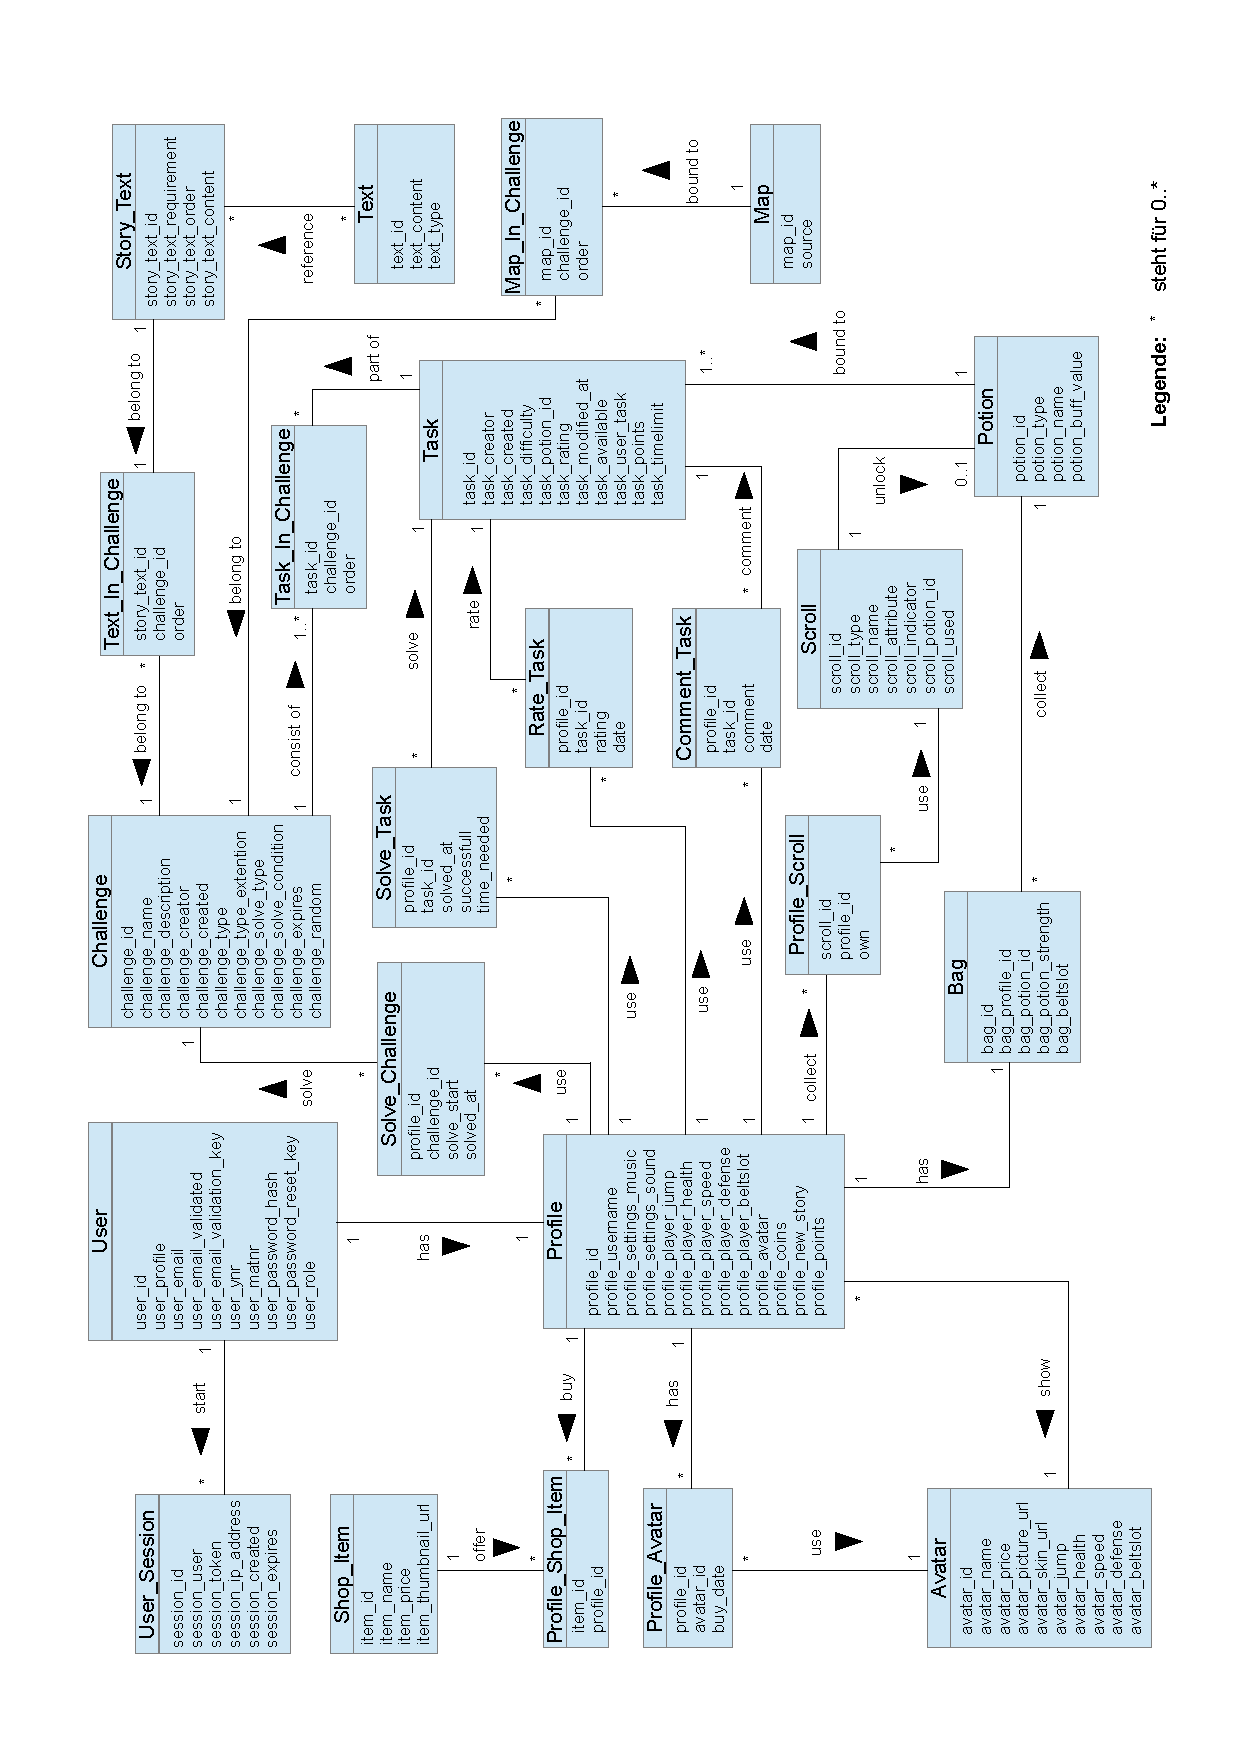
\includegraphics[width=1.0\textwidth]{figures/Klassen-Diagramm-final.pdf}
\caption{Klassendiagramm zum SQL-Alchemist}
\label{datenmodell}
\end{figure}
\newpage
\newpage



%
%
%\end{center}
%
%\end{entity}

%!TEX root = ../Fachentwurf.tex

% Kapitel 7
%-------------------------------------------------------------------------------
\chapter{Konfiguration}
Für den SQL-Alchemist benötigen wir weder einen Rechner, noch einen Server mit einer bestimmten Konfiguration. Aus diesem Grund wird an dieser Stelle nicht weiter auf diesen Punkt eingegangen.

Außerdem existieren auch keine config-Dateien auf die an dieser Stelle hingewiesen werden müsste.
%!TEX root = ../Fachentwurf.tex

\chapter{Glossar}



Lofi-Coins:\\
Lofi-Coins sind die Spielwährung. Diese werden im Minigame erspielt und können genutzt werden, um Avatare und andere Dinge im Ingame-Shop zuerwerben.

Playerstatistics:\\
Attribute des Spielers, die Auswirkungen auf das Minispiel haben (Sprungh\"ohe, Geschwindigkeit, Leben und St\"arke).

Potions: \\
Die im Spiel verwendete Bezeichnung f\"ur Tr\"anke, die dem Spieler tempor\"are Vorteile
verschaffen. Sie werden durch das richtige Bearbeiten von SQL-Anfragen erstellt werden k\"onnen. 

Scrollcollection: \\
Beschreibt den Fortschritt des Spielers indem es die bereits gesammelten Scrolls speichert. 

Scrolls: \\
Einmalig im Spiel im einzusammelnde Objekte. Besitzt man diese, ist man in der Lage durch das L\"osen von SQL-Statements Potion zu erstellen oder die Playerstatistics dauerhaft zu erh\"ohen. 


%------Ende des Dokumentes------------------------------------------------------
\end{document}
